\documentclass[12pt,a4paper]{article}
\usepackage[a4paper]{geometry}
\usepackage{array}
\usepackage{hhline}
\usepackage{graphics}
\usepackage{csvsimple}
\usepackage[russian,english]{babel}
\usepackage[utf8]{inputenc}
\usepackage[T2A]{fontenc} 
\usepackage{ulem}
\usepackage{cmap}
\usepackage{makecell}
\setlength\extrarowheight{2pt}
\setlength{\parindent}{0cm}
\newcommand{\phylentry}[6] {\\\hline\makecell{
#1\medskip\\
\hhline{|-|}
\\#2\\#3}
&\makecell{#4}&\makecell{#5}}
%Syntax: \phylentry{Who}{When}{Where}{Phylosophy}{NotPhylosophy}{ETC} // currently ETC is not used
\hoffset -1.6cm 
\textwidth  16.5cm 
\textheight 24cm 
%\topmargin -1cm 
\parskip 8pt 
\setlength{\unitlength}{1cm}
\sloppy
\addto\captionsenglish{
\renewcommand{\contentsname}{{\bf CO}ntents}
\renewcommand{\refname}{Bibliography}
\renewcommand{\figurename}{Figure}
\renewcommand{\tablename}{Table}
\renewcommand{\abstractname}{Abstract}
\renewcommand{\partname}{Section}
\renewcommand{\bottomfraction}{0.5}
\renewcommand{\floatpagefraction}{0.4}
\renewcommand{\textfloatsep}{0.5cm}
\renewcommand{\intextsep}{0.6cm}
\renewcommand{\floatsep}{0.3cm}
}

\renewcommand\theadalign{cb}
\renewcommand\theadfont{\bfseries}
\renewcommand\theadgape{\Gape[4pt]}
\renewcommand\cellgape{\Gape[4pt]}
\begin{document}
%..................................................................
\begin{titlepage}
\par 
\vspace*{-2cm}
\begin{center}
{\sf \Large
\vspace*{1.5cm}
{\Huge Семенов, 8-й семестр, 2017}\\
{ Все, что вы хотели {\small(или не хотели, но сдавать надо)} знать о философии,\\ но боялись спросить}}\\
\vspace*{2cm}
\scalebox{1.2}{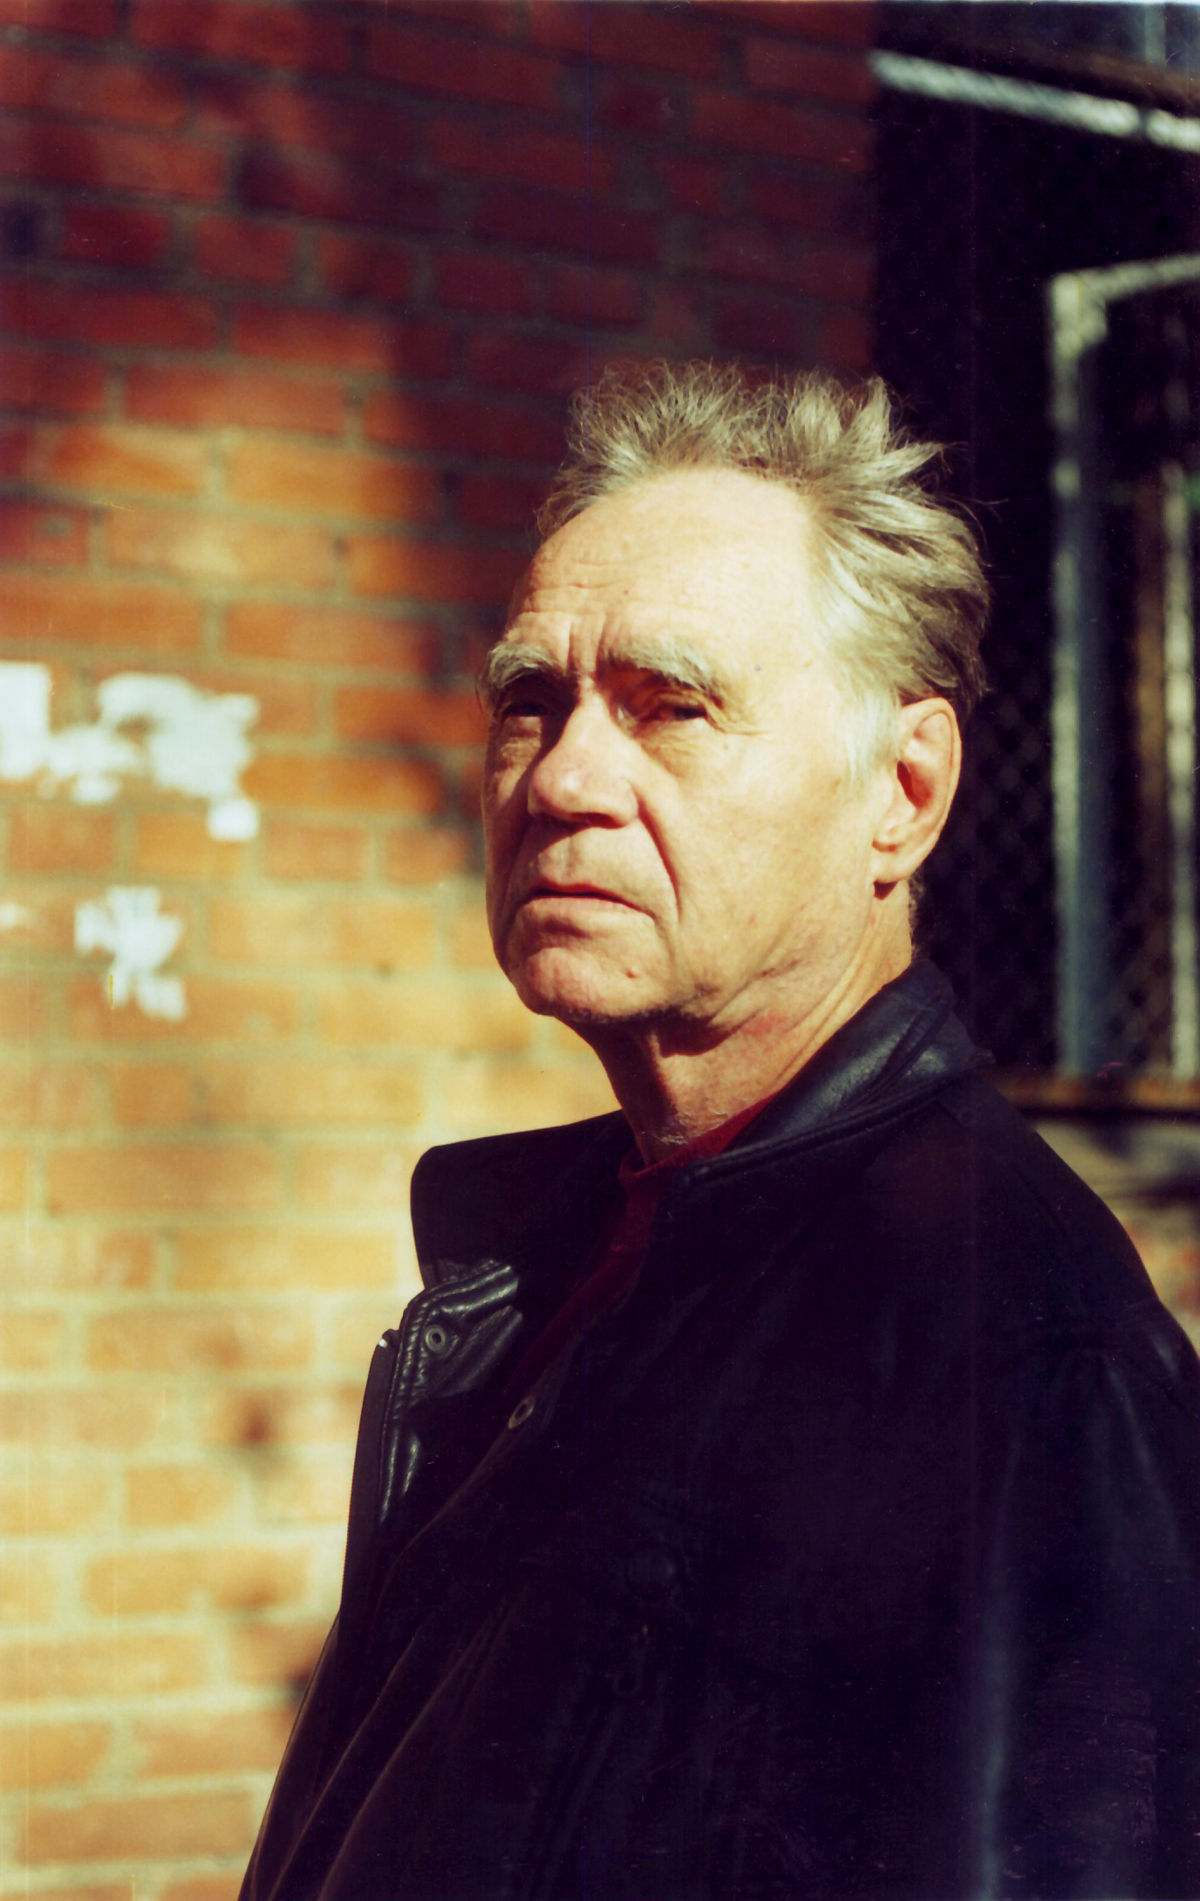
\includegraphics{thegod.png}} 
\begin{flushright}
\sl\small
by Nyaxx11k aka KingKO,\\
Institute for Porn and Pederasts,\\
Chair of Roosterology
\end{flushright}
\end{center}
\end{titlepage}
%..................................................................
\topmargin -1cm 
\hoffset -0.7in 
\textwidth 6.0in 
\textheight 9.0in 
\normalsize 
\pagenumbering{arabic}
%----------------
\tableofcontents
\pagebreak
%----------------

\section{Истина как цель научного исследования. Истина и заблуждение.}
Согласно т.н. "Классическому определению истины", \textbf{истина} - это то, что согласуется с действительностью. \textit{Т.е. соответствие между миром и сознанием}.
Соответственно \textbf{заблуждение} - то, что с действительностью не согласуется. \textit{Заметьте, заблуждение, а не ложь. Ложь - это отрицание истины исключительно в матлогике. В остальных науках это - умышленное введение в заблуждение.}
Ясно, что все науки занимаются поиском истины.
Каждая из них ищет истину о чем-то своем: биология - о живых организмах, физика - о предельно общих законах природы и т.д.

\section{Истина как объект философского исследования.}
Ясно, что все науки занимаются поиском истины.
Каждая из них ищет истину о чем-то своем: биология - о живых организмах, физика - о предельно общих законах природы и т.д.
\textbf{Философия} же ищет истину о самой истине: как достичь истины, не свалившись в заблуждение - изучает методы познания истины.

\section{Философия как теория познания и самый общий метод мышления.}
Философия ищет истину о самой истине: как достичь истины, не свалившись в заблуждение.
То есть философия является теорией познания (\textbf{гносеологией}/\textbf{эпистемологией}).
По другому задача философии может быть сформулирована так: как мыслить правильно, т.е. так, чтобы прийти именно к истине.
А это означает, что философия - всеобщий метод познания и наиболее общий метод мышления. 

\section{Понятие объекта и субъекта, объективного и субъективного}
\textbf{Субъект} - это существо, обладающее сознанием и волей, и способное к целенаправленной деятельности,
которую оно направляет на \textbf{объект} - некий предмет/явление.
У нас в курсе деятельность - это познание.
Т.е. субъект познает объект.
\textit{Да, субъект может быть и объектом. Семенов грозился просить привести примеры объектов.
Да, называем все, что видим, и будет счастье.} 
Соответственно, вводят понятия \textbf{субъективного} - оно означает, что что-то зависит от субъекта,
и \textbf{объективного} - того, что от субъекта не зависит.

\section{Ступени человеческого познания}
У человека есть два способа познания - \textbf{чувственное познание} и \textbf{мышление} (ака \textbf{умственное познание}).
Первое осуществляется органами чувств и человеку неподвластно.
А второе - это человеческая деятельность, она подвластна сознанию, а значит, и методологию для нее можно разрабатывать (более того, это-то и есть философия как метод мышления).

\section{Чувственное познание. Его основные формы.}
У чувственное познания три стадии:
\begin{enumerate}
\item \textbf{Ощущение} - начальная фаза. Объект воздействует на субъекта, и его органы чувств (всего их 5) передают информацию об этом в мозг. \textit{Вопрос на засыпку: назовите наши чувства. Ответ: зрение, слух, обоняние, осязание, вкус, \sout{интуиция}. Очень смешно. Интуиция - это к Аль-Газали. Или к РЕН-твшникам}.
\item \textbf{Восприятие} - на этой ступени данные со всех органов собираются в единый образ предмета.
\item \textbf{Представление} - образ ранее воспринятого предмета может быть воспроизведен в сознании субъекта и в отсутствии этого предмета.
\end{enumerate}
Это познание есть не только у человека, но и у любых животных. Понятно, что чувственного познания не достаточно для того, чтобы познать закономерности мира.

\section{Мышление как деятельность человека. Проблема правильного образа (метода) познания. Философия как метод мышления и наука о мышлении - логика}
\textbf{Мышление} - это уже человеческая деятельность, она подвластна сознанию, а значит, и методологию для нее можно разрабатывать, в отличие от чувственного.
Более того, этим-то и занимается философия.
Значит, философия является еще и наукой о мышлении - логикой. Вообще, \textbf{логика} - это наука
о мышлении, в центре внимания которой - его правильность или истинность.\textit{ Далее мы увидим, что не все - философия, что логика.
} Следует оговориться, что его она изучает как способ достижения истины, т.е. не интересуется, например, отклонениями в мышлении \textit{(это к психиатрам)} \textit{ При мышлении органы чувств не используются непосредственно. }

Главный компонент мышления - \textbf{понятия} (\textit{нет, не те, по которым живут на зонах, хотя эти "Понятия" - это понятие}). Далее, из понятий собирается \textbf{суждение} (\textit{-Пример суждения? -Кит синий!}). Из них можно выводить новые суждения путем умозаключений, не наблюдая за процессом. \textit{Кит - петух. Петух - синий. $\Rightarrow$ Кит синий. Бред? Ну, формально все ОК. Кстати, петух скорее голубой...}


\section{Два вида мышления: рассудочное и разумное, и две логики: формальная и содержательная (философская)}
Мышление может быть как субъективной деятельностью - \textbf{рассудочным мышлением},
так и объективным процессом - \textbf{разумным мышлением}. 
У каждого из них логика своя - соответственно, \textbf{формальная} и \textbf{содержательная}.
Формальная логика изучает лишь правильность мышления, а посему от философии с проблемами истины она давно отпочковалась, став самостоятельной наукой. Логика же разумного мышления в философии используется интенсивно. 
\textit{ Это не значит, что философия забивает на чувственное познание и рассудок, и уж тем более, что она их отрицает. Очевидно, для работы разума нужны как чувственные данные, так и рассудок - чтобы стать известными, результаты работы разума в любом случае нужно перевести в формы, присущие рассудку.}

\section{Классическое определение истины}
Без лишних предисловий: \textbf{Истина} - это то, что согласуется с действительностью (\textit{by Платон/Аристотель-у первого оно встречается раньше, но приписывают обычно второму}). 
Т.е. иначе говоря, истина - соответствие между миром и сознанием.

\section{Проблема определения понятий "мир" и "сознание"}
Обычно дают определение через род и видовое отличие. Мир и сознание - предельно общие понятия, еще более общее только одно - бытие (т.е. и мир, и сознание - есть): но это нам ничего не даст - бытие и так все включает. Значит, придется раскрывать отношение - что из них первично, что вторично. Тем самым, кстати, автоматом определятся оба. Это - \textbf{"основной вопрос философии"}. 

\section{Основной вопрос философии}
Обычно дают определение через род и видовое отличие. Мир и сознание - предельно общие понятия, еще более общее только одно - бытие (т.е. и мир, и сознание - есть): но это нам ничего не даст - бытие и так все включает. Значит, придется раскрывать отношение - что из них первично, что вторично. Это - \textbf{"основной вопрос философии"}. Именно по ответу на него классифицируют направления философии. \textit{Кстати, философ, считающий, что нет никакого основного вопроса - недофилософ и петух. Считающий, что на вопрос нет и не будет ответа - это уже другое.}

\section{Философия как мировоззрение (онтология). Натурфилософия. Социальная философия.}
Итак, определить мир и сознание можно только одним образом - раскрыв отношение между ними. Это значит, что тем самым будут определены оба понятия. Тем самым философия дает еще и предельно общий взгляд на мир, т.е. является \textbf{онтологией}. Раньше, когда науки еще были в зачаточном состоянии, только философия была готова дать хоть какую-нибудь картину мира. Такое учение называется \textbf{натурфилософией}. В настоящее время натурфилософия отмерла за ненадобностью. \textit{Но не онтология - она по прежнему занимается проблемами мира - теми, которые нужны для теории познания}. Но кроме природы есть еще общество - им занимаются \textbf{социальная философия} и \textbf{философия истории}. И с ними все не так однозначно, как с натурфилософией. Во-первых, есть \textbf{общественное сознание} - в широком смысле это все знание человечества; более того, сознание отдельного человека формируется в обществе \textit{(а дети-Маугли ни говорить, ни социализироваться не могут)}. Во-вторых, разные школы придерживаются разных взглядов на общество: первые говорят, что общество - только название, а на самом деле есть только взаимодействующие люди. Вторые таки признают общество. Это два направления - \textbf{социальный номинализм} и \textbf{социальный реализм} соответственно.

\section{Материализм как онтология и как гносеология. Понятие материи.}
Итак, первое направление в философии \textit{(кстати, именно его и придерживается Семенов)} - это \textbf{материализм}: первичен мир, сознание вторично. Причем сознание отражает мир. Т.о. материализм признает объективную реальность - \textbf{материю}. 

\section{В чем заключается вторичность сознания по отношению к материи.}
Нельзя сказать, что материалисты объявляют, что сознания нет вообще. Просто сознание не образует отдельного мира, оно зависимо от материи и не существует без нее. Действительно, сознание - продукт мозга, который есть ни что иное, как материя. Но это не самое главное. А самое главное в том, что сознание - \textsl{отражение} материи.

\section{Формы материализма. Натурматериализм и панматериализм.}
Материалисты до Маркса были непоследовательны: в природе они были материалисты (\textbf{натурматериалисты}) при переходе к обществу им приходилось переходить на позиции идеализма. Действительно, казалось бы, общество - это отражение сознания людей. 
\textit{Еще бы, общество в отличие от физических тел не пощупаешь.}
\textit{Не говоря уже о том, что общество в отличие от мира не вечно - оно возникло вместе с людьми.} Маркс же нашел социальную материю - производственные отношения. Тем самым материализм стал полным -\textbf{панматериализмом}, или \textbf{диалектическим материализмом}. Другое важное его следствие - человек не просто пассивный наблюдатель, он воздействует на мир, преобразуя его.

\section{Субъективный идеализм. Солипсизм. Трудности субъективного идеализма.}
Итак, идеализм дает прямо противоположный материализму ответ: сознание первично, мир вторичен.  Первый его сорт - \textbf{субъективный идеализм}: мир существует только в моем сознании. Представитель такого течения - Беркли (правда, на старости лет он ушел в объективные идеалисты).\textit{Тут так же, как и с материалистами: мир не отрицается, а существует как комплекс моих восприятий}. Люди тоже существуют в моем сознании как духи.
Точка зрения, когда мир есть лишь форма существования моего сознания, называется \textbf{солипсизмом}. Т.е. все, что не воспринимается, не существует. Что происходит с миром, когда я его не ощущаю (сплю, например)? Беркли вкрутился тем, что ввел других мыслящих духов, которые воспринимают мир в мое отсутствие (\textit{"Стоп, люди же тоже должны пропадать, когда я сплю... А, неважно"}) А как мои представления отличать от восприятия? Очевидно, что воображаемым яблоком наесться нельзя. Вот тут и приходится вводить абсолютный дух, который бы отделял представление от восприятия. А это уже попахипает \textbf{объективным идеализмом}. Точнее, им и является. \textit{Другие пытаются отгородится софизмами.} Но субъективный идеализм - не просто глупость. Это, скорее, раздувание до неприличия одного из моментов отношения сознания и объективного мира.

\section{Объективный идеализм. Суть и основные компоненты.}
Итак, идеализм дает прямо противоположный материализму ответ: сознание первично, мир вторичен. Его второй сорт - \textbf{объективный (абсолютный) идеализм}. Его фундамент заложен еще пифагорейцами и Платоном, из тех, кто поновее - Шеллинг и Гегель. Чтобы избавиться от багов солипсизма, вводят \textbf{абсолютный дух}, который бы отделял представление от восприятия. Этот дух - вне человека и человечества. Он творит (мыслит) природу. А духи людей уже отражают эту природу. Итого насчитываются три источника и три составные части объективного идеализма:
\begin{enumerate}
\item Абсолютный дух
\item Природа
\item Остальные духи (люди тут).
\end{enumerate}
\textit{Абсолютный дух кажется похожим на Бога, но мешать идеалистов и верунов нельзя - Семенов опустит тут же! И поделом: философия и религия - две большие разницы. Здесь и далее, вплоть до христианской философии, слово "Бог" означает скорее "абсолютный дух", чем "бородатый дяденька на небе, запиливший этот мир за семь дней (или за шесть?)"}

\section{Социоконструктивный идеализм}
Его основоположник и ярчайший представитель - Фихте. Центральное понятие у него - Я. \textit{Еще один субъективный идеалистишка? Как бы не так!} Этот Я - общественный разум, творящий мир. Это не Я индивидов, и даже не их прямая сумма. Это - объективный дух по отношению к людям. Но в отличие от объективных идеалистов, Я не существует без индивидов. Это абсолютное Я творит не-Я.

\section{Монизм. Два его вида: материализм и идеализм}
Нам потребуются понятия \textbf{субстанции} и противоположного ему \textbf{акциденции}. 
\textbf{Субстанция} - это бытие, существование которого не обусловлено никаким другим бытием,
находящимся за его пределами.
А \textbf{акциденция} - это бытие производное, имеющее началом
что-то отличное от него самого. Теперь философские течения можно классифицировать по числу субстанций. Материализм и идеализм - \textbf{монизмы}, т.е. у них только одна субстанция (материя или дух соответственно). \textit{Есть еще монисты - маргиналы, у которых субстанцией является не мир и не сознание, а что-то еще: ощущения/жизнь/экзистенция. Вроде этих петушков можно свести к идеалистам, если вычистить словоблудие, прикрываемое терминами.}

\section{Понятие субстанции и акциденции}
\textbf{Субстанция} - это бытие, существование которого не обусловлено никаким другим бытием,
находящимся за его пределами.\\
\textbf{Акциденция} - это бытие производное, имеющее началом
что-то отличное от него самого.

\section{Дуализм и плюрализм}
Напомню, \textbf{субстанция} - это бытие, существование которого не обусловлено никаким другим бытием,
находящимся за его пределами,
а \textbf{акциденция} - это бытие производное, имеющее началом
что-то отличное от него самого. \textbf{Дуализм} - это философское течение с двумя субстанциями. Его сторонником был, к примеру, Декарт. У него мир (протяженная субстанция) отдельно, сознание (мыслящая субстанция) отдельно. Но мыслящую субстанцию он делил на Бога и человеческую душу. А Бог создал все, в том числе и протяженную субстанцию, а потом просто забил на нее. Т.е. она и не очень-то и субстанция. Таким образом, Декарт не стоял целиком на позициях дуализма, а был эклектиком - с уклоном в объективный идеализм. 

А \textbf{плюрализма} - течения с более чем двумя субстанциями, придерживался Лейбниц. Правда, у него градус эклектики был не ниже - вводя субстанции - монады, которые вечны, он вводит также и Бога, который их все же может уничтожать и создавать. 


\section{Агностицизм (феноменализм)}
Наконец, есть течение, утверждающее, что человечество не знает ответа на основной вопрос, и не узнает никогда. Это - \textbf{агностицизм} ака \textbf{феноменализм}, и его создатель - Юм \textit{(вообще-то он Хьюм - Hume)}. Основное положение - если мы знаем вещь, то она находится в нашем сознании. Следовательно, вещи вне нашего сознания непознаваемы. Чтобы ответить на основной вопрос, нам нужно выйти за рамки нашего сознания. \textit{Не путать со скептиками-они не отрицают познаваемость, а только сомневаются}.


\section{Позитивизм: первый, второй и третий. Постпозитивизм. Аналитическая философия.}
\textit{Черти, причем очень популярные - Бертран Рассел, Карл Впоппер - это все сюда. Семенов говорит, что это наиболее популярная философия, по крайней мере, на Западе.}
\begin{enumerate}

\item 1-я волна. Конт, Милль, Спенсер.
\textit{Хотели очистить философию от метафизики. В результате - дикая эклектика.} 
Выделяли три стадии человеческого познания - теологическую (все объяснялось богами), метафизическую (все через магию), и позитивную - там у нас есть чувственное познание, а все вне чувств непознаваемо.
\item 2-я волна ака \textbf{эмпириокритицизм}. Авенариус, Мах.
Мешанина из субъективного идеализма и агностицизма. Вводят "элементы мира", и объявляют, что все вещи из них состоят. В результате эти элементы оказались ощущениями. \textit{Ленин их в своем "Материализме и эмпириокритицизме" прямо на первой странице отправил под шконку.}
\item 3-я волна ака \textbf{неопозитивизм}. Родился из \textbf{аналитической философии} (Мур, Рассел, Витгенштейн), которая основной целью ставила  анализ языка (ибо чувственные данные у них становятся подлинными, когда в языковую форму запаковываются). Представители - Карнап, Франк, Гедель, Шлик. Это также известно как \textbf{логический позитивизм}, некоторые даже отделяют его от аналитической философии. \textit{Рухнул с позором, родив только чайник Рассела на орбите.}
\item \textbf{Постпозитивизм} (Поппер, Кун, Лакатос, Фейерабенд). Критиковали неопозитивистов.
\textit{Хули они взамен предлагали, Семенов нам не говорил, но в книжке своей пишет:\\
"...Возникший в результате кризиса неопозитивизма новый вариант позитивизма —
постпозитивизм в лице, если не всех, то по крайней мере ряда его крупнейших
представителей, встал на путь прямой дискредитации науки. Тенденции, отчетливо
наметившиеся в работах Т. Куна (1922-1996), нашли свое завершение в сочинениях
П. Фейерабенда (1924-1994). Согласно утверждениям последнего, теории науки
имеют нисколько не больше ценности, чем мифы, сказки, религиозные учения. А
раз так, то наука ни в коей мере не может быть использована для опровержения
феноменализма. Так, философское направление, объявлявшее себя ни мало ни
много, а философией науки, превратилось в конце концов в теоретическое
обоснование и оправдание любых лженаучных построений и вообще любого
мракобесия, включая религиозное..."\\
Короче, позитивизм - курятник.
}
\end{enumerate}

\section{Основные эпохи истории человечества.}
\begin{enumerate}
\item Зарождение человека - 1.9 млн лет назад
\item Современный человек появился 40 тыс. лет назад.
Тогда было только житейское знание и \textbf{первобытный коммунизм} - общество было бесклассовым.
\item Потом появилась цивилизация  - уже с \textbf{классами}. Ее основные признаки - монументальные сооружения и письменность.
31 век д.н.э-9 век д.н.э - \textbf{эпоха Древнего Востока}. Представлена в основном Древним Египтом и Шумерами (потом уже появились Индская цивилизация, Шань и гипотетическая Ся).
Там возникла преднаука - знание уже собиралось и фиксировалось, но анализа причин и доказательств не было.
Строй там был интересный - Маркс назвал его "\textbf{азиатский}", Семенов же называет его \textbf{политарным}. Некоторые историки говорили, что там был рабовладельческий строй, но это неверно - рабы там не играли роли.
\item 8 в.д.н.э-5 в.н.э. - \textbf{Античная эпоха}. Там появилась наука, философия, и там было \textbf{рабство}.
\item 6 в.н.э-15 в.н.э. - \textbf{Средневековье}. Там \textbf{феодализм}.
\item 16 в.н.э-1914/1917 - \textbf{Новое Время}. Там \textbf{капитализм}.
\item 1914/1917-наше время - \textbf{Новейшее время}. Там все еще пока \textbf{капитализм}.
\end{enumerate}
\textit{Напомню - \textbf{частная собственность}-это собственность, позволяющая одним людям эксплуатировать других. С \textbf{личной собственностью} ее путать нельзя.}

\section{Возникновение классового общества. Эпоха Древнего Востока. Общественный строй Древнего Востока. Появление письменности и преднауки.}
\textbf{Эпоха Древнего Востока} была в 31 век д.н.э-9 век д.н.э. В нее появилась \textbf{цивилизация}-классовое общество, города, монументальные сооружения и письменность (пока - в виде иероглифов на камне/папирусе). Тем самым знание стало фиксироваться. Это еще не наука, потому что анализа знанй, поиска причинно-следственных связей и доказательств не было - только готовые рецепты (\textit{"А вывести формулу можете? Нет? На пересдачу!"}). Знание было общим - содержало и астрономию, и медицину, и математику. Строй там интересный был. Маркс назвал его "\textbf{азиатский}", Семенов же называет его \textbf{политарным}. При нем есть работники и управляющие. Средства производства принадлежат управляющим, но не каждому по отдельности а все всем сразу. \textit{Поэтому-то в СССР и говорили, что в эту эпоху было рабство. Уж больно похожи госпредприятия и номенклатура на Древний Египет. Семенов характеризует строй СССР как \textbf{индустриальный политарный}.}

\section{Античное общество и античная эпоха. Возникновение в античном мире теоретического мышления, философии и науки.}
Говоря об античной эпохе (8 в.д.н.э-5 в.н.э.), нужно первым делом упомянуть Древнюю Грецию. Это было не цельное государство, а скорее сеть из ~260 полисов, разбросанных по Греции, Италии, побережью Средиземного Моря и его островам. Т.е. от северной Африки до южной Франции и побережья Черного моря. Там было \textbf{рабство} - захваченные на войне люди лишались всех прав и отправлялись на работы. За 6-7 лет человек изнашивался и умирал.  Политические режимы в Греции были разнообразными - от \textbf{тирании} до \textbf{демократии}. Именно в Древней Греции появились науки, в т.ч. философия, и теоретическое мышление. Это произошло следующим образом - греки многому научились у египтян. Но египтяне создали лишь преднауку  - доказательств у них не было. \textit{Еще бы, запруфай-ка теорему Пифагора на иероглифах! Греком с алфавитным письмом  в этом плане было явно полегче.} А еще у них были литература и театр.

Второе важное государство - это Древний Рим. Рим возник еще в 8-м веке д.н.э., однако влияние он стал набирать только в 3 в. д.н.э., уже после развала империи Александра Македонского. Тогда Рим был республикой. Потом, уже в 1-м веке д.н.э., появилась Римская Империя. Ее развал (или, скорее, раскол на Западную и Восточную) империи в 476 году н.э. считается концом античности.

\section{Милетская школа. Проблема, которую она стремилась решить.}
%\ \ \ \
\underline{Фалес ($\approx$624 д.н.э - $\approx$546 д.н.э.)}. Город: Милет, Малая Азия.

Математик, астроном, философ. Первый доказал теорему (\textit{да-да, ту самую, про параллельные прямые и угол}). \textit{Использовал формальную логику еще до того, как Аристотель ее завершил, и она стала мейнстримом}. Предсказывал затмения. В плане философии же - основатель \textbf{Милетской школы}, да и вообще \textbf{философии}. Считал, что в мире есть первовещество, и все сущее - его проявления. Фалес считал это первовещество \textbf{водой} (\textit{скорее, это нечто абстрактное, текучее и жидкое, а не буквально вода из моря}). А так как все движется и меняется, то есть и движущая сила - \textbf{душа, "психе"}.

\underline{Анаксимандр ($\approx$619 д.н.э - $\approx$546 д.н.э.)}. Город: Милет, Малая Азия.

Создатель первых солнечных часов, первой карты.
Считал, что в мире все движется по единым законам (\textit{а вот и детерминизм подъехал!}). Человек у него - потомок морских животных, а мир имеет вид вращающегося цилиндра. Его осколки улетели и образовали звезды и Солнце с Луной. Причем таких цилиндров бесчисленное множество, мы - на одном из них.
По его мнению, в мире есть первопричина, первовещество. В отличие от Фалеса, считал им нечто неопределенное -т.н. \textbf{апейрон}. Он неосязаем и доступен только уму.

\underline{Анаксимен ($\approx$585 д.н.э - $\approx$525 д.н.э.)}. Город: Милет, Малая Азия.

У него мир имеет вид неподвижного диска. 
Первовеществом у него был \textbf{воздух}, превращающийся во все остальное в результате разрежения и сгущения.

Главный же вопрос - мир вечен, но в нем нет ничего вечного. Что же делает мир вечным? Именно это и было причиной введения первовещества. Сходные взгляды высказывал \underline{Гераклит}. Его и милетцев иногда даже объединяют в \textbf{Ионийскую школу}.

\section{Гераклит Эфесский.}
%\ \ \ \
\underline{Гераклит ($\approx$540 д.н.э - $\approx$480 д.н.э.)}. Город: Эфес, Малая Азия.

Как и милетцы, считал мир вечным, в котором нет ничего вечного. Тоже вводил первовещество - на этот раз \textbf{огонь}: "Мир был, есть и будет огнем, вечно разгорающимся и утихающим". Но интересен он также тем, что видел движущую силу в противоречивости этого мира (\textit{по типу "нож-это оружие, но в руках хирурга он спасает жизни и т.д."}). Получается, мир состоит не из набора вещей, а из процессов. Гераклит назвал это \textbf{диалектикой} - мир - это вечный процесс. 

\section{Пифагор и пифагорейцы.}
%\ \ \ \
\underline{Пифагор ($\approx$570 д.н.э - $\approx$487 д.н.э.)}. Родился на острове Самосе, но жил и работал в южной Италии.

Сторонник аристократии. свалил сначала с Самоса с его тираном Поликратом, а потом из Кротона после демократического переворота.
Основатель пифагорейской школы. Доказал теорему имени себя.

Выделял три вида духовных ценностей - религию, этику и науку. Пифагор и пифагорейцы чуть ли не обожествляли числа: все явления - это числа. \textit{Да, кстати, цифры зримы, а числа нет. Они идеальны. И они управляют миром. Все в мире - проявление мира чисел. Это - зайчатки объективного идеализма, отделения слова от понятия. Да, и Матрицы (или урматов). Правда, это все-таки зачатки.} Мир описывали как центральный огонь (\textit{не Солнце}), вокруг которого вращаются десять сфер: пять планет, Земля, Солнце, Луна, Млечный путь и Антиземля (чтобы всего было десять). Делили все на десять пар противоположных понятий, например: "четное-нечетное", " мужское-женское", "четырехугольное-многостороннее","свет-тьма" и т.д. \textit{Да, а почему пифагорейцы начали придавать огромное значение числам? Все пошло от музыки и экспериментов со струнами, которые они проводили - уж очень впечатлили их гармоники. Вот и полезли искать везде след чисел.}

\section{Элейская школа. Основные ее представители. Учение Парменида о бытии. Вклад элеатов в развитие философской мысли.}
%\ \ \ \
\underline{Ксенофан ($\approx$580 д.н.э - $\approx$490 д.н.э.)}. Бродячий певец родом из Малой Азии, обошел всю Грецию. \textbf{Пантеист}-отождествлял Бога и природу, бытие. Мифологию Древней Греции не признавал, считал выдумкой людей.

\underline{Парменид ($\approx$546 д.н.э - $\approx$470 д.н.э.)}. Город Элея, это в Италии.

\scalebox{0.38}{
\includegraphics{COmic-parmenides.jpg}}

Что такое бытие? Это - то, что есть. А небытие? То, чего нет. Раз так, то бытие вечно, иначе откуда оно пришло и куда уйдет? В небытие? Так некуда, получается. А раз так, то и в мире ничто не появляется и не исчезает и не меняется. Итого есть только неподвижное и единое (иначе два бытия отграничены небытием) бытие, а наши чувства нас обманывают. А это, кстати, уже важная мысль - Парменид поделил познание на чувственное и умственное. \textit{И напоследок: раз чувства нас обманывают, какое-то движение подсовывают, то истину необходимо постигать \textbf{разумом}, а в наблюдении подтверждения мы не найдем}.

\underline{Зенон Элейский \textit{(не путать с Китийским-тот был стоик!)} ($\approx$490 д.н.э - $\approx$430 д.н.э.)}. Ученик Парменида, доказывал своего учителя \textbf{апориями} - парадоксами, из которых следовала невозможность движения. До нас дошло не все. Например: "Летящая стрела неподвижна, так как в каждый момент времени она занимает равное себе положение, то есть покоится; поскольку она покоится в каждый момент времени, то она покоится во все моменты времени, то есть не существует момента времени, в котором стрела совершает движение." Или про Ахиллеса, черепаху и сходимость рядов.

\underline{Мелисс ($\approx$485 д.н.э - $\approx$425 д.н.э.)}. Его важнейшее положение - бесконечность мира не только во времени, но и в пространстве. Опять же, явления - видимости, а есть только сущности.



\section{Эмпедокл и Анаксагор.}
%\ \ \ \
\underline{Эмпедокл ($\approx$492 д.н.э - $\approx$430 д.н.э.)}. Жил на острове Сицилия.

Вводил четыре элемента: огонь, воду, землю и воздух. Они вечны, а все сущее - результат смешения этих стихий под действием двух сил - \textbf{дружбы и вражды}. \textbf{Редукционист} - новые вещи у него - лишь смесь старых качеств. История у него разбита на 4 фазы:
\begin{enumerate}
\item Вначале была дружба
\item Потом появилась вражда, но влияние дружбы еще решающее
\item Потом только вражда
\item И наконец, происходит переход от вражды к дружбе. Мы именно в эту эпоху и живем.
\item GOTO 1
\end{enumerate}
У него было много интересных мыслей - про конечность скорости света, про естественный отбор (правда, это было скорее соединение нежизнеспособных органов в монстров, которые в итоге стали гармоничными и способными к размножению). А ощущение он понимал так: частицы стихий стряхиваются и попадают на наши органы чувств.

\underline{Анаксагор ($\approx$496 д.н.э - $\approx$428 д.н.э.)}. Родился в Клазоменах, Малая Азия. Переехал в Афины, был другом Перикла, который даже спас его от кары за безбожие.

У него есть семена мира - \textbf{гомомерии}, их, в отличие от Эмпедокла, бесчисленное множество. Сами по себе они неподвижны. Движущая сила, объединяющая их - \textbf{ум (нус)}. Т.е. тела - просто смешение семян мира. Пытался создать теорию чувственного познания, основанную о том, что органы чувств дают представление о мире, но не о гомомериях. 

\textit{Но это еще не атомизм. И у одного, и у второго, стихии были бесконечно делимы.} 

\section{Древнегреческий атомизм. Возникновение абсолютного детерминизма.}
%\ \ \ \
\underline{Демокрит ($\approx$460 д.н.э - $\approx$360 д.н.э.)}. Город: Абдеры, во Фракии.

Ярчайший представитель \textbf{атомистического материализма}.
Ученик Левкиппа, который и предполагается как создатель сего направления \textit{(но увы и ах, данные неточные)}.
Его взгляды неясны до конца - возможно, его точка зрения менялась в процессе. Основные же положения:
есть пустота, небытие. В ней есть мельчайшие неделимые частицы - \textbf{атомы}\textit{(Неделимые? Резерфорд, Кюри и Майтнер под столом.)}. Эти атомы обладают весом, формой и незримы. Из них-то все и состоит. Атомы разбросаны по всей пустоте - миров много. Да, и чувства нас опять-таки обманывают. Мир не такой, как в сознании. \textit{Типа, сладкое - это гладкий атом на язык попал}. Чувственное познание у него называется темным, а познание разумом - светлым. Считал, что темное познание - необходимая ступень, но дальше можно и без нее. \textit{Говорят, на старости лет даже глаза себе выколол, чтоб постигать мир исключительно разумом}. И важнейшее его открытие - \textbf{детерминизм}. Атомы подчиняются всеобщим законам, а значит, все имеет причину и предопределено, а случайность - только от незнания причины. Необходимость тоже всеобщая. \underline{Эпикур} впоследствии взял атомизм на вооружение, но детерминизм отвергал - у него была случайность и свобода воли.

\section{Софисты. Протагор и Горгий.}
Софисты были в 6-5 вв д.н.э. Они были профессиональными ораторами. Обучали риторике и философии, ибо умение отстоять свою точку зрения было необходимо (демократия-выборы, суды без прокуроров/адвокатов). Умели доказать что угодно.
\textit{\\-Это собака - твоя?\\ -Ну да, я ее хозяин.\\-А она часом не мать?\\-Ну мать, вон у нее щенки бегают.\\-Ага, значит она твоя и мать. Значит, ты - сукин сын. q.e.d.}\\
Подразделяются они на старших и младших. Протагор и Горгий - оба старшие.

\underline{Протагор ($\approx$486 д.н.э - $\approx$411 д.н.э.)}. Город: Абдеры, во Фракии.

Считал, что человек - мера всех вещей. А раз так, то и у каждого своя правда. Истина есть то, что приносит пользу. А полезность субъективна. Выделял две стадии человечества - естественную  и человеческую.

\underline{Горгий ($\approx$480 д.н.э - $\approx$380 д.н.э.)}. На протяжении жизни жил в Италии, Афинах, умер в Ларисе. 

Горгий in a nutshell:
\begin{enumerate}
\item Ничто не существует.
\item Если же и существует, то не познаваемо.
\item Ну а если и познаваемо, то языком непередаваемо.
\end{enumerate}

\textit{Короче, в этих учениях образ жизни софистов виден насквозь}.

\section{Сократ.}
%\ \ \ \
\underline{Сократ ($\approx$469 д.н.э - $\approx$399 д.н.э.)}. Афинянин.

 Книг не писал, вел беседы (называл методику \textbf{майевтикой} - искусством повивальной бабки): вначале включал иронию, и когда оппонент понимал, насколько безблагодатная у него точка зрения, Сократ наводящими вопросами помогал ему родить мысль. Был обвинен в развращении молодежи и богохульстве. Приговорен к казни и выпил яду.

Что же касается его философских воззрений, то он считал, что человек - единство души и тела, причем первую управляет вторым. Суть человека в душе, а значит, воспитать человека - это воспитать дух. Знания у него тоже таятся в душе, а добродетель проистекает из знания.\textit{"Никто не желает зла по своей воле - оно творится чисто по незнанке"}. Спорами восстанавливал авторитет истины, опущенной софистами. 
Тремя главными добродетелями считал мужество, справедливость и умеренность. Говорил, что круг потребностей нужно ограничить, чтобы не зависеть от других людей (эту мысль развили \textbf{киники}).

\section{Платон.}
%\ \ \ \
\underline{Платон (Аристокл) ($\approx$427 д.н.э - $\approx$348 д.н.э.)}. Афинянин, но после смерти Сократа покинул Афины. Создатель философской школы - Академии. Родоначальник эстетики.

Первый законченный \textbf{объективный идеалист}. Он отделил слово от понятия: первое материально, второе идеально. Задавшись вопросом о том, существует ли общее в реальном мире, пришел к идее, что есть мир вещей и мир идей, а существование понятия трояко: в вещах, голове, и мире идей. Идеи вечны, а вещи приходят и уходят, а посему и материальный мир не вечен. В рассказе про пещеру сравнивал идеи с реальными объектами, а вещи - с тенями от этих объектов. У человека есть душа, она вечна и пребывает в мире идей, если не находится в теле. Высшая идея - благо. Душа вспоминает идеи, которые она видела в том мире - отсюда у нас есть какие-то понятия (например, о том же благе и красоте).
У него есть и вечная материя, из которой состоят невечные вещи. И еще у него есть Бог, который, руководствуясь идеями, творит мир из материи. Душу человека делил на три: ощущающую, пылкую и разумную. Первые две сравнивал с конями, а третью - с извозчиком.

У него есть классификация государственных строев: власть одного (царь/тиран), власть группы (аристократия/олигархия), власть большинства (демократия). Описывал трехклассовое идеальное общество - правители-философы, стражи, крестьяне-ремесленники. \textit{Первая утопия. Поппер за это на него наехал. Ну что от Впоппера еще ждать?}

\section{Аристотель.}
\underline{Аристотель ($\approx$384 д.н.э - $\approx$322 д.н.э.)}. Родился в Стагире, жил в Афинах. Путешествовал по Греции. Воспитатель Александра Македонского. Прошел Академию, но впоследствии основал свою школу - Ликей (Лицей). Бежал из Афин после смерти Александра Македонского.

Геоцентрист, считал, что есть 55 небесных сфер. На Земле все состоит из огня/воды/земли/воздуха, и так до орбиты Луны, а все,что выше - эфир. 
Разрабатывал учение о силлогизмах. У него есть рассудок и разум. У рассудочного мышления есть три формы
\begin{enumerate}
\item Понятие. \textit{Береза, кошка, дом и т.д.}. Оно не истинно/ложно.
\item Суждение (\textit{Береза - дерево; петух - не человек}). Выражается предложением и уже несет истину/заблуждение. Но не всякое предложение выражает суждение (\textit{На пересдачу!/Не в свои сани не садись!}). 
\item Умозаключение - из суждений делаем еще одно. 
\end{enumerate}
Завершил формальную логику - три закона:
\begin{enumerate}
\item Тождества - понятие употребляется в одном и том же значении.
\item Противоречия -"Не противоречь сам себе"
\item Исключения 3-го: или А, или не-А истинно - третьего не дано. 
\end{enumerate}
Открыл дедукцию/индукцию.
Остальное - см. ниже.

\section{Учение Аристотеля о бытии.}
Вводил 10 основных категорий, в порядке убывания важности:
\begin{enumerate}
\item Сущность/Субстанция - она делится на две - совокупность всех отдельных вещей и виды с родами. \textit{Род - что-то общее, вид - более конкретное}.
\item Количество - любая вещи имеет количественную характеристику.
\item Качество - делится на признак и состояние. \textit{Исчезает призкак- исчезает и предмет, а состояние же - временное}
\item Положение
\item Место
\item Время
\item Отношение
\item Обладание
\item Претерпевание/Страдание
\item Движение
\end{enumerate}
Мира идей не было - критиковал Платона. Общее у него есть только в голове и вещах. 

Движение у него присуще бытию. Осуществляет его Бог.
В результате движения возникают новые вещи. Вводил 4 типа причин
\begin{enumerate}
\item Материальная - из чего
\item Формальная - что
\item Действительная/Производящая - откуда 
\item Целевая - ради чего. Вводил понятие \textbf{энтелехии} - внутренней силы, потенциально заключающей в себе цель и окончательный результат.
\end{enumerate}
по которым возникают вещи. Где движение, там энергия, его осуществляющая. Есть 6 форм движения
\begin{enumerate}
\item Перемещение
\item Рост
\item Уменьшение
\item Качественное преобразование
\item Возникновение
\item Исчезновение
\end{enumerate}
Выделял три типа души - растительная, присущая всему живому, чувственная, присущая животным, в том числе хомо сапиенсу, и разумная, присущая человеку. Душа не привязана к телу, управляет им и не зависит от него.

\section{Учение Аристотеля о материи и форме.}
У Аристотеля было понятие материи, которая вечна. Из нее состоят все вещи. Но материя сама по себе пассивна, она лишь возможность вещей: чтобы образовать вещь, она должна соединиться с формой. Форма тоже вечна. Бог - высшая форма.

\section{Теория познания Аристотеля.}
Существует объективный мир, не зависящий от воли и сознания человека. В нем есть вещи, действующие на органы чувств человека - этих органов выделено пять, как обычно.
Разделял чувственное познание и мышление. Чувственное дает знания лишь об отдельных вещах, а мышление - уже об общем. У него было два разума - пассивный человеческий и активный божественный. 
В человеческом есть общее знание, которое извлекается миром и активным разумом. 

\section{Учение Аристотеля об обществе.}
Из работ Аристотеля об обществе мало что дошло. Из того что дошло: делил режимы на 6 категорий:
\begin{enumerate}
\item Царизм/Тирания - власть одного в интересах всех/его самого.
\item Аристократия/Олигархия - власть группы в интересах всех/ее самой.
\item Полития/Де(рь)мократия  - власть среднего классы/толпы.
\end{enumerate}
В каждой группе первый режим хороший, второй плохой. \textit{Потом произошел сдвиг в терминах: полития стала демократией, а демократия - охлократией.}
Делил общество на три слоя - богачи, средняки, бедняки. Их интересы противоположны друг другу - а это уже зачатки идей о классовой борьбе. Сам Аристотель был на стороне средняков. \textbf{Соц. реалист} - считал, что общество организм, движущийся по своим законам. Выделил три ячейки общества - семью (\textit{с родителями, детьми, и, естественно, рабами - впитал-таки предрассудки строя. По Марксу-с!}), селение (группа семей) и полис (группа селений).

\section{Философия в эпохи поздней классики и эллинизма.}
После Аристотеля философия была уже не та. Поздней классикой называют 4 век д.н.э. Далее, уже после смерти Александра Македонского, идет эпоха эллинизма (до 30 года д.н.э., после которого Рим уже всех нагнул). Перечислим основные направления:
\begin{enumerate}
\item Киники. Центральная мысль - идея независимости путем ограничения потребностей (первой ее высказывал Сократ).
\item Эпикурейцы. Демокритовский атомизм, ну уже без детерминизма.
\item Стоики \textit{не стояки - это к Диогену!}. Зародилась в Греции, но и в Риме была популярна. Была идея о полной предопределенности, а свобода состояла в том, чтобы подчиниться судьбе.
\item Скептики. Сомнение и невозмутимость. \textit{По легенде, скептик Пиррон назвал идеалом своего направления свинью, которая во время шторма сидела на корме и невозмутимо жрала из корыта.}
\item Разгулялись \textbf{эклектики}  - заимствующие разные идеи из разных школ, иногда даже не заботясь о согласованности учения.
\end{enumerate}
Детально они обсуждаются в вопросах 60-63.


\section{Киники}

Они же циники. Ядро их философии - нужно быть независимым от других, для чего свои потребности нужно свести к минимуму. Это нужно, чтобы стать счастливым.
Противники рабства. Делили состояния человечества на природное и государственное, причем второе - хуже.

\underline{Антисфем (435 д.н.э.-370 д.н.э.)}. Создатель направления.

\underline{Диоген (390 д.н.э.-323 д.н.э.)}. Экстравагантный товарищ. Жил в бочке (глиняном кувшине, если быть точным). \textit{Поговаривал "Ох, вот бы и голод унять поглаживанием живота", онанируя. Прямо. Посреди. Главной, мать ее. Площади. Афин. Афинян в основном и за людей не считал - настолько они, по его мнению, были тупые. Это он принес Платону ощипанного петуха в качестве контрпримера к определению человека.}

\scalebox{0.8}{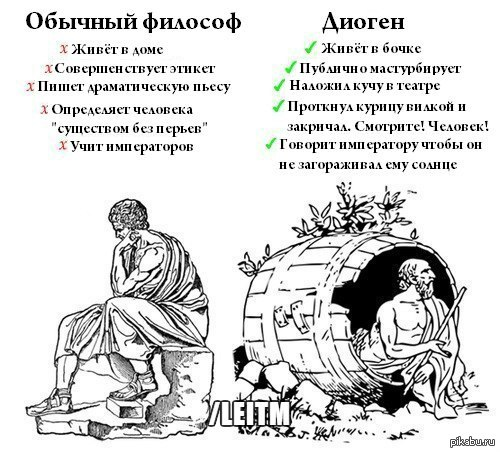
\includegraphics{diogen}}

\section{Эпикур и эпикурейцы}
%\hspace{8pt} 
\underline{Эпикур (341 д.н.э.-279 д.н.э.)}. Родился на Самосе, жил в Афинах.
Философию делил на логику (учение о познании), физику (учение о природе) и этику (учение об общественной жизни). \textbf{Атомист}, но отказался от детерминизма. Атомы без случайности просто бы падали вниз, не образуя вещей. Считал благом наслаждение, а злом страдание, при этом не сводился к гедонизму: есть потребности
\begin{enumerate}
\item Естественные необходимые - их удовлетворять нужно
\item Естественные не необходимые и
\item неестественные не необходимые. Тут уже следует проявлять умеренность и ограничивать
\end{enumerate}
Наивысшее наслаждение - беседа с мудрецом. Добродетели у него - апатия, бесстрастие, невозмутимость.

\underline{Тит Лукреций Кар (99 д.н.э.-55 д.н.э.)}. Последователь Эпикура. Написал книгу "О природе вещей", в которой и расписал его взгляды (возможно, с добавлением собственных).

\section{Стоицизм}
%\hspace{8pt} 
\underline{Зенон Китийский \textit{(не путать с Элейским!)} (334 д.н.э.-262 д.н.э.)}. Создатель направления. Был купцом с Кипра, корабль разбился, стол философом в Афинах. 

\underline{Хрисипп(280 д.н.э.- 205 д.н.э.)}. Город: Солы. Еще один стоик.

Те же составные части философии, что и у Эпикура. Сравнивали ее с яйцом: логика - скорлупа, физика - белок, этика - желток.
У них есть пассивная материя и дух, приводящий ее в движение. Существует цепь причин и всеобщая предопределенность. Свобода у них, тем не менее, тоже есть. Человек может свободно подчиниться судьбе, а может упираться, но в конечном итоге все все равно свершится как надо. У Стои 3 эпохи:
\begin{enumerate}
\item 4-3 вв д.н.э - ранняя Стоя
\item 2-1 вв д.н.э - средняя Стоя
\item 1-3 вв н.э. - поздняя, или римская Стоя
\end{enumerate}
Мир у них делится на две части - зависящая от меня (мои мысли), и независящая от меня.
Что зависит - тем занимаемся, что не зависит - игнорим. Это учение - \textbf{Учение об адиафоре}.
Поздняя Стоя - см. ниже.

\section{Скептицизм}
%\hspace{8pt} 
\underline{Пиррон (365 д.н.э.-275 д.н.э.)}. Пелопоннесец.

\underline{Тимон (320 д.н.э.-230 д.н.э.)}. Те же идеи.

Философ у них ищет счастье в жизни. Для этого ему нужно ответить на три вопроса:
\begin{enumerate}
\item Из чего состоят вещи, и чем они друг от друга отличаются?
\item Как мы к ним относимся?
\item Как нам извлечь из них пользу?
\end{enumerate}
А мы-то и не знаем, в чем отличие, а потому должны воздержаться от суждений. Хотя мы можем сказать, что вещь кажется там такой-то. Но одно дело видимость, а другое - сама вещь. Т.о. допускаем все возможное и не волнуемся - вот и счастье.

\section{Философия в эпоху Римской державы.}
Эпоха Римской державы - последняя эпоха античности. Помимо классической философии, появляется еще и христианская, которая, правда, часто сводилась к богословию. Христианство зародилось в 1 в.н.э. (\textit{искренне ваш, капитан Очевидность})среди низов, как коллективная воля народа к справедливости. Призывала к смирению, ибо Боженька на небе всех рассудит. Была принята на вооружение правящим классом - в 313 году н.э. император Константин уравнял в правах христианство и религию древнего Рима (\textit{а что, это отличный опиум для народа получился - до сих пор юзают.}). Опять же, просто перечислим основные направления:
\begin{enumerate}
\item Эклектики, например Цицерон (он больше по ораторству был).
\item Поздняя стоя. 
\item Неоплатонизм.
\item И христианская философия, в той ее части, в которой она не сводилась к тупому богословию.
\end{enumerate}


\section{Римская Стоя (Сенека, Эпиктет, Марк Аврелий)}
%\hspace{8pt} 
\underline{Луций Анний Сенека  (6 д.н.э.-65 н.э.)}. Воспитатель Нерона. Крупный администратор. В 41-49 годах находился в ссылке. Как и Сократ, покончил с собой по приговору суда.

Стоик. Не соглашался с Сократом в том, что знание дает добродетель. Не считал зазорным быть богатым, но богатство у него должно служить людям. У него тоже есть мир из пассивной материи, и дух, состоящий из божества и судьбы. 

\underline{Эпиктет (55 н.э.- 130 н.э.)}. Еще один стоик. Был рабом, получил вольную. Странствовал по Албании и вел беседы. Раб у него может быть свободным, а господин - рабом. Главное счастье - быть невозмутимым и свободным. Есть объективный мир, неподвластный человеку, и подвластный ему духовный мир. Значит, надо приспособить себя.

\underline{Марк Аврелий Антонин (121 н.э.-180 н.э.)}. Император. Говорил, что жизнь бренна и кратковременна. Призывал к смирению.


\section{Неоплатонизм}

Основано на Платоне.

\underline{Аммоний Саккас}. Александриец. Основатель.

\underline{Плотин (206 н.э.-275 н.э.)}. Ученик предыдущего. 

У него есть понятие единого духовного первоначала. Из него получаются божественный ум и божественная душа (в порядке убывания ранга).  Дальше - природа, материя, пронизанная формой. И наконец человек (\textit{Еще ниже только петух. Сарказм же.}) из разума, души и тела. Душа бывает разумной и чувственной. Чтобы добиться экстаза (первоначала), нужно подчиниться судьбе.

Еще там была Сирийская школа:

\underline{Ямвлих}. Основатель. Богослов, культист, первосвященник. 

И Афинская школа:

\underline{Порфирий} осознал проблему общего и отдельного. И еще \underline{Прокл}. Он был, и больше ничего. \textit{Вот и иллюстрация тождества бытия и ничего у Гегеля}.


\section{Христианская философия. Патристика.}
\textit{Минздрав предупреждает: чрезмерное употребление религии вредит рассудку и разуму.}

\underline{Тертуллиан (155 н.э.-225 н.э.)}. Карфагенец. Критик античной философии - язычники же все. Выразил концепцию Троицы. Верует, ибо абсурдно - говорил, что веру пруфать нельзя. 

Подъехали \textbf{патристики} - "отцы церкви", ХГМ-направление в философии.

\underline{Климент Александрийский (150 н.э.-220 н.э.)}. Считал, что христианство можно доказать, используя достижения античной философии.

\underline{Ориген (185 н.э.-254 н.э.)}. Те же взгляды, что и у предыдущего. Еретик, ибо ставил Бога-Отца выше Сына - сын все-таки должен родиться.
 
После 313 г. свобода мысли улетучилась, и патристика начала загибаться.

\section{Августин Аврелий и его философия истории.}
%\hspace{8pt} 
\underline{Августин Аврелий ака Блаженный/святой Августин (355 н.э.- 430 н.э.)}. 

\textbf{Патристик}. Создал первую философию истории. Она конечно, далека от реальности, но все же: Бог наметил план истории, и история подстраивается под него - \textbf{провиденциализм}. Есть Град земной - в нем живут по плоти, и Град божий - там живут по духовным ценностям (\textit{с христанутостью это не скоррелировано!}). На Страшном Суде их пихают в Ад и Рай соответственно. Государство он приравнивал к банде, но считал это зло необходимым. Источник бедствий у него двоякий - рушится град земной, пополняется град божий. Концепция у него унитарная - человечество движется как единое целое. Но прогресса нет, а будет только конец света. Периодизировал историю так:
\begin{enumerate}
\item Адам-Ной
\item Ной-Авраам
\item Авраам-Давид
\item Давид-Вавилонское пленение
\item Вавилонское пленение-Христос
\item Христос-Страшный суд. Дальше - светлое будущее на небе (или вечный DOOM). Думал, что это произойдет, когда Рим грохнется.
\end{enumerate}


\section{Гибель античного мира. Философская мысль на заре средних веков. Северин Боэций, Аврелий Кассиодор. "Семь свободный искусств". }
Начали образовываться варварские государства. Римская империя рухнула в 476 году, хотя де-факто она распалась раньше. В Италии воцарился Теодорих, король остготов. 

\underline{\sout{Синерим Оэтский}Северин Боэций (480-524)}. Был приговорен к казни за участие в заговоре, в тюрьме написал книгу "Утешение философией", в которой занимал позиции стоиков. Утверждал, что Бог знает будущее, но это не отменяет свободной воли индивида. Мышление делил на разумное и рассудочное. Перевел все труды Аристотеля о логике на латынь.

\underline{Аврелий Кассиодор ($\approx$485-$\approx$585)}. Создал монастырь, а при нем библиотеку с античными текстами. Создатель концепции "Семи свободных искусств". Они делись на две ступени -  \textbf{тривиум}:
\begin{enumerate}
\item Грамматика
\item Риторика
\item Диалектика (по сути, это и есть философия)
\end{enumerate}
и \textbf{квадривиум}:
\begin{enumerate}
\item Арифметика
\item Геометрия
\item Музыка
\item Астрономия
\end{enumerate}

\section{Каролингское возрождение. Иоанн Скот Эриугена.}
После крушения Римской империи с философией было все плохо - богословие подменяло ее. Но тут пришел Карл Великий, и запилил империю из всей Европы, кроме Англии (800 г.) \textit{Империю, Карл, империю!} В эпоху правления Карла Великого - Каролингское возрождение - наступил подъем. 

\underline{Иоанн Скот Эриугена (810-877)}. Ирландец. Жил и работал при дворе Карла Лысого - следующего за первым Карла. С примесью  богословия, но все-таки философ. Наследник патристики. Ставил знание выше веры. То, что все знание содержится в Библии, означает, что его нужно уметь подчерпнуть оттуда. Считал, что общее существует - был \textbf{реалистом}. Считал, что есть три формы существования общего: 
\begin{enumerate}
\item В божественном разуме \textit{(Платоновский мир эйдосов, естественно, пошел нах)}
\item В вещах
\item В голове человека
\end{enumerate}

\section{Становление феодализма.}
После распада Каролингской империи начались изменения в обществе, приведшие к созданию нового строя - феодализма (10-11 вв). Это был синтез цивилизованных остатков структур Римской империи и варварского строя Германии. 
Он основан на собственности на землю. Крепостные крестьяне уже не были рабами (Например, нельзя было убить крепостного. Правда, можно засудить и казнить.); но феодализм возможен и без них. Были также и крестьянские общины. Крестьянин платил помещику оброк или отрабатывал его на барщине. Землю можно было брать в аренду - так появились сеньоры и вассалы. Крестьяне часто восставали, а посему вассалы обращались за военной помощью к сеньору. Сеньор тоже имел право затребовать у вассалов помощь. В западной Европе осталась одна централизованная структура, обладавшая властью - католическая церковь.  


\section{Возникновение городов и городской культуры в Западной Европе. Монастырские, епископальные и городские школы.}
10-11 вв. ознаменовались окончательным утверждением феодализма. 
%В 12-м веке стали использоваться механизмы - часы, водяные и ветряные мельницы. 
В западной Европе осталась одна централизованная структура, обладавшая властью - католическая церковь.
Города становились все более и более независимыми; возникают городские общины, собственный аппарат принуждения у городов и т.п. Да, и городской воздух делал крестьян свободными. В городах расплодились ремесленники, юристы и купцы.
Возникла потребность в образовании. В городах стали появляться школы и университеты; последние обладали автономией. Еще школы были при монастырях. Изучали там семь свободных искусств$^\mathtt{TM}$, право и юриспруденцию. Да, и философия, стало быть, в школах тоже была. Ее назвали \textbf{схоластикой}. 

\section{Ранняя схоластика: Ансельм Кентерберийский, Иоанн Росцелин, Пьер Абеляр, Иоахим Флорский}
В 11 веке появилось направление в философии, именуемое \textbf{схоластикой}. 

\underline{Ансельм Кентерберийский Д'Аоста. (1033-1109)}. Глава английской церкви.

Веру ставил выше знания: да, без знания никуда, но оно служит вере. Придумал \textbf{онтологическое доказательство} существования Бога: \textit{"Бог есть нечто, превосходящее по величине (величию) все мыслимое. Если атеист говорит «Бога нет», то он думает о Боге. В этом случае нельзя не признать, что Бог существует хотя бы в его уме в момент мысли. Отрицая, атеист хочет сказать, что Бога нет вне его ума, то есть в реальности. Однако в Боге как существе абсолютно совершенном, сущность совпадает с существованием (см. выше). Значит, если в нашей мысли есть понятие о Боге, то Он с необходимостью существует в реальности. Если же мы допускаем нечто мыслимое, больше Бога, то приходим к противоречию (так как изначально было определено, что Бог превосходит все мыслимое) и уже не понимаем, о чем говорим. Бог – это Высшее бытие, более которого ничего не существует, именно поэтому ничего более него невозможно помыслить. Мы мыслим о Нем, потому что он существует, а не наоборот. Однако это вовсе не значит, что если любое другое понятие кроме Бога (например, сказочный остров) существует в мысли, то оно существует в реальности. Отождествление понятия мысли с его реальным существованием применимо только в отношении Бога. Потому что Он – Высшее совершенство, чья сущность с необходимостью совпадает с существованием. Все же остальные вещи получают свое существование от Бога."} (\textit{софист долбаный!}). \textbf{Реалист} - считал, что общее существует  - это план, по которому Бог создавал этот мир; а также в вещах и в сознании (\textit{привет, Иоанн Скот Эриугена})


\underline{Иоанн Росцелин (1051-1122)}. 

А этот- \textbf{номиналист}. Общие понятия - только слова, и ничего более. Даже мышление на этой почве отрицал.
Больше его работ не дошло, т.к. был еретиком.

\underline{Пьер Абеляр (1079-1142)}. 

Тоже \textbf{номиналист}, но уже не такой, как \underline{Иоанн Росцелин}: общее - не только слово, но и понятие. Т.е. оно существует в человеческом сознании. Также ставил знание выше веры. В сочинении "Да и нет" привел противоречия в Библии. Также написал "Историю моих бедствий", хотя это уже не о философии.

\underline{Иоахим Флорский (Калабрийский) ака Джоаккино да Фьоре  (1130-1202)}. 

Делил историю человечества на три эпохи:
\begin{enumerate}
\item Эпоха Бога-Отца: люди живут по плоти, и в повиновении их может держать только рабская покорность.
\item Эпоха Бога-Сына: люди поумнели, и покорность уже не рабская, а сыновья.
\item Эпоха святого духа: люди будут управлять сами собой и наступит свобода. В "Откровениях" Иоанна Богослова вычитал, что это наступит в 1260 году. 
\end{enumerate}
У него были последователи, например, \underline{Томас Мюнцер}, которые отрицали, что царство Бога на Земле (п. 3), само не придет. \textit{Революционненько. Добье-е-емся мы освобожде-е-енья своею собственной руко-о-ой.}
 
Эти люди все признавали необходимость знаний в той или иной мере. Были еще \textbf{иррационалисты}, которые говорили, что знания вообще не нужны (\textit{Этих петушков мы не изучаем}).

\section{Арабы и арабские завоевания. Возникновение ислама и исламского богословия. Возрождение античной науки и возникновение интереса к античной философии в исламском мире. Арабская философия (арабский аристотелизм)}
На востоке были кочевые племена (у них было что-то вроде первобытного коммунизма) и города, уже с классовым обществом.
Кочевые племена охраняли/грабили корованы (sic!). После конца Рима караваны накрылись.
Разрозненным городам следовало бы объединиться, дабы запилить армию и пойти всех нагибать. 
Это было основной предпосылкой возникновения религии. 
В итоге, после пары неудачных попыток, такой религией стал ислам, созданный Мухаммедом из Мекки.
Это монотеистическая религия - нет Акбара кроме Аллаха (и Мухаммед - пророк его). 
Испытал влияние иудаизма и христианства. 
Под ее влиянием, все очень быстро собралось в единое государство. Потом Мухаммед умер, и появились замы Аллаха не земле - халифы и Халифат - исламское государство \textit{(запрещенная в РФ террори... ой да ну на\#@!)}. 
Пошел процесс завоевания: от 2/5 Испании ("Конкиста") до Индии, Индонезии и Филиппин.
Руси тоже досталось - Татаро-Монгольское Иго же. 
Началась арабизация и исламизация. 
Арабы познакомились с античной наукой, и стали переводить тексты. 
Развивается астрономия (навигация в море + вычисление положения Мекки, чтобы молиться на нее), математика, география, алхимия. 
Возникает два центра - Восточный (Дамаск/Багдад) и Западный (Кордовский Халифат в Испании).
Ислам раскололся на суннизм и шиитизм (из-за вопроса престолонаследия), появилось исламское богословие - \textbf{калам}. 
Философия тоже проникла через античные тексты. Особенно велико было влияние Аристотеля - появился арабский аристотелизм. О них см. далее.

\section{Философия на Востоке исламского мира. Аль-Кинди, Аль-Фараби, Ибн Сина, Аль-Газали.}
%\hspace{8pt} 
\underline{Аль-Кинди (800-877)}. Жил в Ираке (город рождения не известен точно - Басра или Куфа. Умер в Багдаде.)

Философ и естествоиспытатель. Первый арабский \textbf{аристотелист}. Уважал знание. Делил познание на три ступени: логику, естественные науки и философию. Вводил космический разум - нечто, что позволяет открывать тайны. Подвергся гонениям на религиозной почве.

\underline{Аль-Фараби (870-950)}. Родился в Казахстане, свалил в Дамаск.

\textbf{Аристотелист}, но с оговорками. Мир, например, не вечен, а создан Аллахом. Религию считал низшей формой знания, облаченной в метафоры для упрощения понимания ее простым народом. А вот философия - это да, это высшая форма знания, для небыдла.

\underline{Ибн Сина ака Авиценна (980-1050)}. Жил в Бухаре.


\textbf{Аристотелист} и даже мир вечен. Бог - это мышление, мыслящее о самом себе. В мир это мышление не вмешивается.
Общее у него существует в божественном разуме, вещах и понятиях (\textit{прям-таки Иоанн Скот Эриугена arab edition}). Медик.

\underline{Аль-Газали (1058-1111)}. Иран, Тус.

Богослов. Аристотелистов обвинял в безбожии, отступлении от Корана, а главным способом познания считал интуицию. Написал "Опровержение" философов.

\section{Философия на Западе исламского мира. Ибн Рушд.}
%\hspace{8pt} 
\underline{Ибн Рушд ака Аверроэс (1126-1198)}. Из Кордовы, это в Испании. Судья.

\textbf{Аристотелист} до мозга костей, продолжатель материалистической линии в трудах Аристотеля, хотя сам говорил, что только комментатор (\textit{ага, комментарий на трактат}). Написал "Опровержение опровержения". Бог - это мышление, мыслящее о самом себе, как у \underline{Ибн Сины}. 
%
Душа у него, правда, неразрывно связана с телом; бессмертия души нет (хотя и говорит о бессмертии человечества). 
%
Вещи не пришли извне, а всегда принадлежали миру (а он вечен). Религия и философия у него - по-разному сформулированная истина, как у \underline{Аль-Фараби}. Родоначальник концепции двойственной истины.


\section{Арабы и развитие научной и философской мысли Западной Европы. Возникновение университетов в Западной Европе.}
В конце 12 века возник первый университет - Болонский. Появился слой из духовенства - преподаватели. У университета была автономия, собственный суд и полиция. Университет делился на факультеты, во главе стояли деканы, из них один был ректор (\textit{с тех пор мало что поменялось}). Факультеты были - младший - на нем 6 лет изучали \textbf{артистику} - те самые 7 свободный искусств, и старшие - богословия, права и медицины (на них учились еще 5-7 лет). Говорили там на латыни и только на латыни. 
А в Испании тем временем началась \textbf{Реконкиста} - пячили мавров - арабов. Арабская философия тогда и проникла в Европу. Особенно в университетах котировался Ибн Рушд - его последователи именовались \textbf{аверроистами}. Через арабов проник и сам Аристотель.

\section{Аристотель и средневековая схоластика. "Золотой век схоластики".}
Аристотель проник в Западную Европу вместе с арабской философией и стал популярен. Церковь его даже запрещала (1-я половина 13 в), но университеты не обратили внимания на это визгливое кукареканье, и продолжили читать Аристотеля. Наступил золотой век схоластики. Появились церковные ордены - \textbf{Францисканцы} (аврелианцы, Аристотеля принижали) и \textbf{Доминиканцы} ("Псы господни", Аристотеля объявили высшим авторитетом). Доминиканцы были кузницей кадров для св. Инквизиции.

\section{Бонавентура и Альберт Великий}
%\hspace{8pt} 
\underline{Джованни Фиданца ака Бонавентура (1221-1274)}. Генерал ордена францисканцев. 

Идеи у него существуют, но высшее познание дано только Богу. Бог - только форма, он не материален; все остальное же - форма + материя. Теология у него во главе всех наук. Противник \textbf{сенсуализма}. Познание у него имеет три формы
\begin{enumerate}
\item Познание вещей, созданных Богом
\item Познание совственной души
\item Слияние с Богом
\end{enumerate}
%Вера, естественно, выше знания.


\underline{Альберт Великий  ака Альберт фон Больштедт ака Doctor Universalis (1206-1286)}. По происхождению - немец, но учился в Падуе, потом ездил и преподавал. Вступил в Доминиканский орден.

Считал, что необходимо знать греческую философию. Философию и богословие различал. 

\section{Фома Аквинский}
%\hspace{8pt} 
\underline{Фома Аквинский (1225-1274)}. Тоже вступил в Доминиканский орден. Ученик \underline{Альберта Великого} 

У него две истины - разума и откровения. Однако эти две истины отличаются только по форме. Важны и знания, и откровения. Но философия таки обслуживает веру, и вера важнее знания.  Утверждал, что есть недоказуемые и непостижимые для человеческого разума истины. Бог у него - дух, создавший мир из ничего. Ввел еще доказательства бытия Бога:
\begin{enumerate}
\item Существует цепь причин. Что есть первопричина? Б-г.
\item Мир в движении. Кто есть перводвижитель? Б-г.
\item В случайности есть доля необходимости (почему именно так?). Что она такое? Б-г.
\item Есть все более и более совершенные существа. А самое совершенное? Б-г.
\item В мире есть цель, целесообразность. Кто ее задал? Б-г.
\end{enumerate}
Есть естественное познание - вне бытия человека, которое дает нам конкретные вещи. Высшее же познание  - духовное, которое в бытии человека, и только оно дает нам общее. Общее у него опять имеет троякое бытие (см. Иоанн Скот Эриугена).
\textbf{Соц. реалист} - общество у него существует. В обществе неизбежно неравенство. Монархист - пусть король владеет телом, а церковь - душой.
Его философия - \textbf{томизм} - в пропатченном виде и поныне юзается церьковью.

\section{Сигер Брабантский и Роджер Бэкон}
Это пошли аверроисты.

\underline{Сигер Брабантский (1235-1284)}. Француз. Как еретик, подвергся гонениям.

Душа смертна, человечество бессмертно, чудес нет, истина двойственна, знание выше веры.
 
\underline{Роджер Бэкон (1214-1294)}. Окончил Оксфорд, свалил в Париж. Тоже подвергся гонениям, лишен права преподавать, арестован, умер в тюрьме. Францисканец.

Критик феодального строя. Философия, по его мнению, должна давать путь к познанию. Уважал математику и оптику. "Знание - сила" - это он сказал. Считал скорость света конечной. Знание у него из трех источников:
\begin{enumerate}
\item Авторитет. Церковный авторитет и Аристотель. Они могут заблуждаться.
\item Ум. Перерабатываем знания других, делаем выводы. 
\item Опыт. Это безошибочный источник.
\end{enumerate}

\section{Иоанн Дунс Скот и Уильям Оккам}
%\hspace{8pt} 
\underline{Иоанн Дунс Скот (1266-1308)}. Окончил Оксфорд. Преподавал в Оксфорде, Париже, а умер в Кельне. Францисканец.

Завершил теорию двух истин - теперь между ними нет ничего общего. Религия недоказуема, богословие не наука. 

%Душа смертна, человечество бессмертно, истина двойственна. 
\textbf{Реалист} - общее есть, но науки движутся от общего к отдельному. Отдельное у  него - важнее общего. \textbf{Сенсуалист}, но мышлением пренебрегать нельзя. Следуя \underline{Северину Боэцию}, признавал и то, что Бог все знает, и свободу воли.  
 
\underline{Уильям Оккам (1285-1349)}. 

Сбежал от церкви к Людвигу Баварскому, защищал его философией (в те времена был конфликт между церковью и светской властью). Доказывал, что папство - временный институт, а духовная власть должна быть у христианской общины. \textbf{Крайний номиналист} - познание у него интуитивное (т.е. чувственное), которое дает только отдельное. А дальше есть уже вторичное абстрактное познание. Истины тоже две, и они разные. В честь него назвали Бритву Оккама.

\section{Эпоха Возрождения. Ее значение в истории человечества.}
Грань между Средневековьем и Возрождением условна. Обычно ее проводят по границе 15-16 века. Расцвели города в западной Европе, поднялась торговля. Рента с крестьян стала браться деньгами. Крепостное право начало отмирать. Возникли прочные экономические связи, а отсюда и политическое единство. Были попытки создать централизованную власть, отсюда феодализм и крепостное право начали терять позиции. Спустя несколько веков таки появились централизованные государства - Англия, Франция, Испания. В Италии и Германии же города подчиняли все окружение - появились города-государства, например Флоренция/Гамбург. Феодальный уклад быстро сменяется там торгово-бюргерским. Возникает антифеодальное движение. В центре новой культуры - \textbf{гуманизма} - человек. Возрождение античной культуры (отсюда и название эпохи). В работах Бруни и Бьендо появились термины "античность" и "новое время". Возникло книгопечатание - книги подешевели и распространились. 

\section{Важнейшие деятели Возрождения в Италии, Голландии, Англии, Германии и Франции}
Пошла эпоха наезда на схоластику. Аристотель, как фундамент схоластов, сдавал позиции и заменялся Платоном

\underline{Франческо Петрарка (1304-1374)}. 
Создатель литературного итальянского. Имел труды по истории.

\underline{Джованни Бокаччио (1313-1375)}. 
Критиковал Средневековые порядки и духовенство в своей книге "Декамерон". 

\underline{Лоренцо Валла (1407-1457)}. 
Указывал на необходимость критики источников (когда, кем, отражает ли действительность), как античных, так и библейских. Разоблачил "Константинов дар" - что Рим с областью якобы были подарены Папе. Мечтал о возрождении античности.

\underline{Пьетро Помпонацци (1462-1525)}. У него была двойственная истина. указывал, что три монотеистические религии - христианство, иудаизм, ислам - противоречат друг другу, а потому хотя бы две -  фейк. Написал "Трактат о трех обманщиках".

\underline{Никколо Макиавелли (1469-1527)}. Политический деятель из Флоренции. Написал книгу "Государь". Мечтал о единой Италии, этой целью оправдывал средства. В книге "История Флоренции" есть мысль об объективности истории.

\underline{Николай Кузанский ака Кребс (1404-1464)}. Кардинал и богослов. Вселенная у него бесконечна, а Земля - не ее центр. Описал отличие рассудка от разума.

\underline{Эразм Роттердамский (1467-1536)}. Филолог и сатирик. Мечтал об освобождении Нидерландов от Испании. С севером прокатило. Написал "Похвальное слово глупости" - глупость (религия) у него там госпожа мира. Глупость диктует богословие. Схоластику критиковал.

\underline{Томас Мор (1478-1535)}. Лорд-канцлер Англии. Бичевал строй Англии и писал про Утопию. Понял, что беда - в частной собственности, из-за нее людей эксплуатируют. На острове Утопия же у него бы чуть ли не коммунизм. Из-за разногласий по поводу англиканской церкви был репрессирован - отрубили голову.

\underline{Ульрих фон Гуттен (1488-1523)}. Написал "Письма темных людей". Настолько смачная пародия на схоластов, что сначала приняли за оригинал.

\underline{Томас Мюнцер (1490-1525)}. В "Великую крестьянскую войну" был предводителем крестьян. Последователь \underline{Иоахима Флорского}, но ждать не хотел.

\underline{Франсуа Рабле (1490-1553)}. Был монахом, но потом сбросил рясу. Написал сатирический роман "Гаргантюа и Пантагрюэль" - удар по схоластике и богословию.

\underline{Пьер де ля Раме (1515-1575)}. Ненавидел богословие, схоластику. Магистерскую защитил, разгромив Аристотеля, правда, с годами стал умереннее, пересмотрел взгляды. Убит в Варфоломеевскую ночь как гугенот (кальвинист).

\underline{Мишель Монтень (1533-1592)}. Был скептик - в том смысле, что требовал проверять все утверждения. Так сомневался в Аристотеле и схоластике. Написал книгу "Опыты".

\underline{Жан Боден (1530-1596)}. Написал книгу "Метод легкого изучения истории". Выдвинул и обосновал концепцию прогресса человечества. Концепция унитарная - развивается все человечество, а не отдельные страны. Искал движущую силу истории.

Плюс еще трое ниже.

\section{Наука в эпоху Возрождения: Леонардо да Винчи, Николай Коперник. Философия Джордано Бруно.}
В 16 веке наконец появилась настоящая, подлинная, стройная наука. 

\underline{Леонардо да Винчи (1533-1592)}. Художник, изобретатель. Человек у него лишь первый из зверей, а душа не бессмертна. Ценил опыт, но и чистый эмпиризм без анализа отвергал. Развивал математику.

\underline{Николай Коперник (1473-1543)}. В книге "Об обращении небесных сфер" ввел гелиоцентрическую систему. Утверждал, что это лишь способ уточнить расчеты (правда, его модель была далеко не идеальна). Церковь это дело проморгала и не забанила вовремя. А зря - Бога пришлось закидывать за орбиту последней известной тогда планеты (кажется, Сатурн). А когда спохватилась, то:

\underline{Джордано Бруно (1548-1600)}. Горячий парень. Безбожник. Нет двух истин - есть только истина разума, а религия - ерундистика. Мир бесконечен, звезды - те же солнца, с планетами и разумной жизнью. Правда, и мировая душа у него была, но это не Бог никаким боком. Естественно, инквизиция такие мысли приветствовала горячо, даже пламенно. Бруно сидел, подвергался пыткам, но от теории не отрекся. В итоге его теория вместе с ним самим была отправлена в топку. \textit{Сволочь ты, инквизиция. Такого человека сгубила!}

\newpage
\section{Аппендиксъ 1: Словарь терминов}
\hspace{15pt}\textbf{Агностицизм} - философское течение, в котором утверждается невозможность дать ответ на основной вопрос (\textit{про мир и сознание}), по причине того, что невозможно познать что-либо за пределами нашего сознания.

\textbf{Акциденция} - это бытие производное, имеющее началом что-то отличное от него самого.

\textbf{Атеизм} -  система взглядов, отрицающих существование богов. \textit{"Атеизм является отрицанием бога и утверждает бытие человека именно посредством этого отрицания" (Маркс)}.

\textbf{Восприятие} - целостный образ предмета внешнего мира.

\textbf{Гносеология} - теория процесса познания истины, теория познания.

\textbf{Деизм} -  религиозно-философское направление, признающее существование Бога и сотворение им мира, но отрицающее большинство сверхъестественных и мистических явлений, Божественное откровение и религиозный догматизм. Большинство деистов полагают, что Бог после сотворения мира не вмешивается в течение событий (как некий великий часовщик, который сделал часы и больше не вмешивается в их ход).

\textbf{Детерминизм} - учение о взаимосвязи и взаимной определенности всех явлений и процессов, доктрина о всеобщей причинности.

\textbf{Диалектика} - многозначненько:
\begin{enumerate}
\item У Гераклита - учение о том, что мир - непрерывный, вечный процесс.
\item В тривиуме - это одна из дисциплин, под которой понималась философия.
\item Также понимается как предельно общий метод мышления.
\end{enumerate}

\textbf{Дуализм} - это философское течение с двумя субстанциями.

\textbf{Заблужение} - противоположность истины, несовпадение между миром и сознанием \textit{Ложь - умышленное введение в заблуждение, в этом отличие.}

\textbf{Идеализм} - философское направление, в котором сознание первично, мир вторичен.

\textbf{Объективный, идеализм} - течение идеализма, в котором присутствует объективный абсолютный дух.

\textbf{Субъективный, идеализм} - течение идеализма, в котором весь мир существует исключительно в сознании субъекта.

\textbf{Социоконструктивный, идеализм} - течение идеализма, в котором роль абсолютного духа играет общественное сознание.

\textbf{Идеальное} - принадлежащее сознанию, нематериальное, духовное.

\textbf{Истина} - это то, что согласуется с действительностью; соответствие между миром и сознанием.

\textbf{Логика} - это наука о мышлении, в центре внимания которой - его правильность или истинность.

\textbf{Материальное} - принадлежащее миру.

\textbf{Материализм} - философское направление, в котором мир первичен, а сознание вторично.

\textbf{Метод познания} - способ достижения истины.

\textbf{Метод мышления} - способ достижения истины.

\textbf{Мышление} - ступень человеческого познания, подвластная сознанию.

\textbf{Натурфилософия} - разновидность философии, которая стремится дать цельную картину мира. 

\textbf{Неотомизм} - доработанная философия Фомы Аквинского. \textit{Попытка соединить томизм м новыми философскими идеями. Рабочая философия католической церкви.}

\textbf{Номинализм} - философское течение, утверждающее что общее или не существует, или существующее исключительно в голове человека.

\textbf{Общее} - принцип бытия всех единичных вещей, явлений, процессов. \textit{Что, звучит криво? FIXME, а то меня уже заколебало}.

\textbf{Объект} - то, что познается, предмет или явление.

\textbf{Объективное} - то, что не зависит от субъекта.

\textbf{Онтология} - учение о сущем; учение о бытии как таковом; \textit{раздел философии, изучающий фундаментальные принципы бытия, его наиболее общие сущности и категории, структуру и закономерности}.

\textbf{Отдельное (единичное)} - конкретные вещи/события.

\textbf{Ощущения} -  начальная фаза чувственного познания, в которой есть только разрозненные данные от органов чувств.

\textbf{Пантеизм} -  религиозное и философское учение, отождествляющее Бога и мир.

\textbf{Позитивизм} - философское направление, отрицающее возможность познания закономерных связей и отношений действительности и ограничивающее роль науки описанием фактов, явлений; философское учение и направление в методологии науки, определяющее единственным источником истинного, действительного знания эмпирические исследования и отрицающее познавательную ценность философского исследования. \textit{Курятник, БЛДЖАД, хотя с точки зрения формальной логики у них все ОК}.

\textbf{Понятие} - элементарная составляющая мышления.

\textbf{Представление} - образ ранее воспринятого предмета, который может быть воспроизведен в сознании субъекта в отсутствии этого предмета; последняя стадия чувственного познания.

\textbf{Разум} - мышление как объективный процесс.

\textbf{Рассудок} - мышления как субъективная деятельность.

\textbf{Реализм} - течение философии, в котором общее существует как нечеловеческое духовное. 

\textbf{Сенсуализм} - течение философии, в котором чувственное познание объявляется единственным источником знаний.

\textbf{Социальная философия} - предельно общий вгляд на общество.

\textbf{Ступени познания} - чувственное познание и мышление.

\textbf{Субстанция} - это бытие, существование которого не обусловлено никаким другим бытием, находящимся за его пределами.

\textbf{Схоластика} - систематическая европейская средневековая философия, представляющая собой синтез христианского (католического) богословия и логики Аристотеля.

\textbf{Томизм} - философия Фомы Аквинского, христианский аристотелизм. \textit{Учение о способах постижения догматов христианской веры}.

\textbf{Фатализм} -  вера в предопределенность бытия; мировоззрение, в основе которого убежденность в неизбежности событий, которые уже запечатлены наперед и лишь "проявляются" как изначально заложенные свойства данного пространства.

\textbf{Феноменализм} = агностицизм.

\textbf{Чувственное познание} - способ познания, который осуществляется органами чувств и человеку неподвластен.

\textbf{Эпистемология} = гносеология.
\newpage
\section{Аппендиксъ 2: Философский бестиариум <WIP>}
{\scriptsize
\begin{tabular}{|c|c|c|}
\hline
\thead{Кто\\Когда и Где}&\thead{Философия}&\thead{Кроме философии}

\phylentry{Фалес}
{($\approx$624 д.н.э - $\approx$546 д.н.э.)}
{Милет, Малая Азия\\\
(Гонял по заграницам)}
{-Мир вечен\\\
-Первовещество-вода}
{-Смотался в Египет, там ботал преднауку\\\
-Первый доказал теорему\\\
-Предсказывал солнечные затмения}{}

\phylentry{Анаксимандр}
{($\approx$619 д.н.э - $\approx$546 д.н.э.)}
{Милет, Малая Азия}
{-Мир вечен\\\
-Первовещество-апейрон\\\
-Мир-цилиндр\\\
-Человек-потомок морских животных}
{-Смотался в Египет, там ботал преднауку\\\
-Первый доказал теорему\\\
-Предсказывал солнечные затмения}{}


\phylentry{Анаксимен}
{($\approx$585 д.н.э - $\approx$525 д.н.э.)}
{Милет, Малая Азия}
{-Мир вечен\\\
-Первовещество-воздух\\\
-Мир-диск}
{ВОИДЪ}{}

\phylentry{Гераклит}
{($\approx$540 д.н.э - $\approx$480 д.н.э.)}
{Эфес, Малая Азия}
{-Мир вечен\\\
-Первовещество-огонь\\\
-Диалектика: мир-вечный процесс\\\
-Его двигатель - противоположности и противоречия}
{ВОИДЪ}{}

\phylentry{Пифагор}
{($\approx$570 д.н.э - $\approx$487 д.н.э.)}
{Остров Самос, Эгейское море\\ (Прямо у побережья Турции)\\\
Кротон, Южная Италия\\\
Метапонт, Южная Италия
}{-Мир вечен\\\
-Первовещество-огонь\\\
-Диалектика: мир-вечный процесс\\\
-Его двигатель - противоположности и противоречия}
{ВОИДЪ}{}

\phylentry{Ксенофан}
{($\approx$580 д.н.э - $\approx$490 д.н.э.)}
{Колофон, Малая Азия \\\
\textit{<Бродяжничал>}\\\
Элея, Южная Италия
}{
-Пантеист\\
-Греческая мифология-фантазия}
{-Бродячий певец}{}

\phylentry{Парменид}
{($\approx$546 д.н.э - $\approx$470 д.н.э.)}
{
Элея, Южная Италия
}{
-Учитель Зенона\\\
-Отрицал небытие\\\
-Бытие-вечно, неделимо и неподвижно\\\
-Разделил чувственное и умственное познание\\\
-Т.к. его учение чувствами непостижимо\\\
}
{-Герой книг Платона\\\
-\textit{Педераст - любил юношей младых}}{}


\phylentry{Зенон Элейский}
{($\approx$490 д.н.э - $\approx$430 д.н.э.)}
{
Элея, Южная Италия
}{
-Апориями доказывал Парменида (всего 40, дошло 9)
}
{ВОИДЪ}{}

\phylentry{Мелисс}
{($\approx$490 д.н.э - $\approx$430 д.н.э.)}
{
Остров Самос\\\
\textit{<Эмигрировал>}\\\
Элея, Южная Италия
}{
-Мир вечен\\\
-Мир бесконечен
}
{ВОИДЪ}{}


\\\hline
\end{tabular}
\begin{tabular}{|c|c|c|}
\hline
\thead{Кто\\Когда и Где}&\thead{Философия}&\thead{Кроме философии}

\phylentry{Эмпедокл}
{($\approx$492 д.н.э - $\approx$430 д.н.э.)}
{
Акрагант, Сицилия\\\
}{
-4 стихии ака корни\\\
-Дружба и вражда как движущие силы\\\
-4 фазы развития, зацикленные\\\
-Стихи бесконечно делимы\\\
-Частички проникают через поры\\\
\ \ \ воздействуя на органы чувств.
}
{
-Теория эволюции через рандомную \\ \ \ сборку органов\\\
-Конечная скорость света.
}{}

\phylentry{Анаксагор}
{($\approx$496 д.н.э - $\approx$428 д.н.э.)}
{
Клазомены, Малая Азия\\\
\textit{<Эмигрировал>}\\\
Афины, Греция\\\
\textit{<Грохнуть хотели>}\\\
Лампсак, Малая Азия
}{
-Гомомерии ака семена мира (их дофига)\\\
-Ум (нус) как движущая сила
}
{ВОИДЪ}{}

\phylentry{Левкипп}
{(5-й век д.н.э)}
{
Абдеры, возможно Милет
}{
-Учитель Демокрита\\\
-Единственное, что известно - был
}
{ВОИДЪ}{}


\phylentry{Демокрит}
{($\approx$460 д.н.э - $\approx$360 д.н.э.)}
{
Абдеры, Фракия
}{
-Атомизм: атомы в пустоте (пространстве)\\
-Атомы незримы, неделимы\\
-Чувства - кажимость, есть атомы\\
-Детерминизм: случайность \\ \ \ - от незнания причин\\
-Познание темное(чувства) и светлое(ум)\\
-Делил на микро- и макромир\\
-Миров великое множество
}
{-По легенде, выколол глаза, ибо уже не нужны\\}{}

\phylentry{Протагор}
{($\approx$486 д.н.э - $\approx$411 д.н.э.)}
{
Абдеры, Фракия
}{
-Человек-мера всех вещей\\
-Истина-в полезности, т.е. для каждого своя\\
-Мир один, но воспринимаем по-разному\\
-Естественная и человеческая стадии развития
}
{-Софиствовал\\}{}

\phylentry{Горгий}
{($\approx$480 д.н.э - $\approx$380 д.н.э.)}
{
Леонтины, Италия\\
Афины, Греция\\
Лариса, Греция
}{
-Ничего нет\\
-А если и есть, то непознаваемо\\
-А если и познаваемо, то в словах невыразимо
}
{-Софиствовал\\}{}

\phylentry{Сократ}
{($\approx$469 д.н.э - 399 д.н.э.)}
{
Афины, Греция
}{
-Единство души и тела\\
-Душа содержит знания\\
-Зло от незнания\\
-Ограничить потребности для независимости
}
{-Майевтика\\
-Книг не писал\\
-Выпил йаду за развращение \\\ \ \ молодежи и богохульство\\
-Я знаю, что ничего не знаю\\
-А другие не знают и этого\\
-Глав. добродетели - умеренность, \\\ \ \ мужество, справедливость
}{}

\phylentry{Платон (Аристокл)}
{(427/8 д.н.э - 346/7/8 д.н.э.)}
{
Афины, Греция\\
\textit{поскитался}\\
Остров, Сицилия\\
Афины, Греция\\
Остров, Сицилия\\\textit{хотел вернуться, неудачно}\\
Афины, Греция\\
}{
-Классификация политических строев\\
-Первый утопист - гос-во философов\\
-Родоначальник эстетики\\
-В 376 г д.н.э. создал Академию\\
}
{
-Первый завершенный объективный идеалист\\
-Мир эйдосов-идей\\
-Высшая идея-Благо\\
-Материя вечна, вещи-нет\\
-Есть Бог, творящий, руководствуясь эйдосами\\
-Душа-вечна, тело-нет\\
-3 Компонента души-Чувственная,\\ \ \  Пылкая,Разумная\\
-Душа припоминает мир эйдосов \\ отсюда у нас общее и врожденные понятия\\
-Рассказ "Пещера"; эйдосы там-реальный мир
}{}

\\\hline
\end{tabular}
\begin{tabular}{|c|c|c|}
\hline
\thead{Кто\\Когда и Где}&\thead{Философия}&\thead{Кроме философии}

\phylentry{Аристотель}
{(384 д.н.э - 322 д.н.э.)}
{
Стагир, Фракия(Македония?)\\\
Афины, Греция\\\
Халкида, Остров Эвбея
}{
-Учение о бытии\\
-10 Категорий\\
-Вещи-из материи\\
-Материя пассивна\\
-Вещь=Материя+Форма\\
-Высшая форма-Бог\\
-Новый вещи-в результате движения\\
-Двигает Бог\\
-Где движение, там и энергия\\
-6 форм движения\\
-4 причины образования вещей\\
-Выделил законы формальной логики\\
-Индукция/дедукция. Под конец изучал\\ \ \  только последнюю\\
-Изучал силлогизмы
}
{
-Воспитывал Искандера ака Александра Македонского\\
-Расклассифицировал строи\\
-3 ячейки общества - семья, селение, полис\\
-Мысли о классовой борьбе\\
-55 небесных сфер, снизу 4 стихии, сверху эфир.
}{}

\phylentry{Антисфем}
{ ($\approx$435 д.н.э.-$\approx$370 д.н.э.)}
{
Афины\\
}{
-Киник (Циник)\\
-\textit{Первый номиналист}\\
-Аскетизм ради независимости
}
{
ВОИДЪ
}{}

\phylentry{Диоген}
{ ($\approx$390 д.н.э.-323 д.н.э.)}
{
Синоп, Турция\\
Афины, Греция\\
Коринф, Греция
}{
-Киник
}
{
-Жил в бочке (точнее, в глиняном кувшине)\\
-Встретился с Александром Македонским;\\ \ Просил не загораживать Солнце\\
-Опровергал Платона петухом\\
-Дрочил посреди главной площади
}{}

\phylentry{Эпикур}
{ ($\approx$341 д.н.э.-$\approx$279 д.н.э.)}
{
Остров Самос, Турция\\
Колофон, Малая Азия\\
Мелитен, Остров Лесбос\\
Лампсак, Турция\\
Афины, Греция
}{
-Делил знание по восходящей на\\ логику, физику, этику\\
-Атомист, НО\\
-Органически вплел случайность в атомизм:\\ \ иначе все бы просто падало\\
-Благо - наслаждение\\
-Но не гедонист - умеренность нужна\\
-Высшее благо-беседа с умными людьми\\
-\textit{Пантеист}
}
{
-Добродетели - апатия, бесстрашие, невозмутимость\\
-\textit{Человек-результат эволюции}
}{}

\phylentry{Тит Лукреций Кар}
{ ($\approx$99 д.н.э.-55 д.н.э.)}
{
Помпеи, Италия\\
Рим, Италия
}{
-Неизвестно, что у него свое,\\ а что-Эпикура
}
{
-Доксограф Эпикура\\
-Написал книгу "О природе вещей"
}{}

\phylentry{Зенон Китийский}
{($\approx$334 д.н.э.-$\approx$262 д.н.э.)}
{
Китион, Кипр\\
Афины, Греция
}{
-Создатель стоицизма\\
-Логика/физика/этика как яйцо\\
-Учение об адиафоре-\\безразличных для достижения счастья вещах\\
-Детерменизм\\
-Свободная воля как \\возможность подчиниться\\
-Философствовали в портике,\\ отсюда и название
}
{
-Был купцом, пока корабль не утонул близ Афин
}{}

\phylentry{Крисипп}
{ ($\approx$280 д.н.э.- $\approx$205 д.н.э.)}
{
Солы, Киликия (над Сирией)\\
Афины, Греция
}{
-Скептик\\
-3 вопроса\\
-Только кажимость\\
-Допускаем все и не паримся
}
{
ВОИДЪ
}{}

\\\hline
\end{tabular}
\begin{tabular}{|c|c|c|}
\hline
\thead{Кто\\Когда и Где}&\thead{Философия}&\thead{Кроме философии}


\phylentry{Пиррон}
{ ($\approx$365 д.н.э.- $\approx$275 д.н.э.)}
{
Элида, Пелопоннес, Греция\\
Афины, Греция
}{
-То же, что и у Зенона Китийского
}
{
-Доксограф Эпикура
-Написал книгу "О природе вещей"
}{}

\phylentry{Тимон}
{ ($\approx$320 д.н.э.- $\approx$230 д.н.э.)}
{
Флиунт, Пелопоннес, Греция\\
Афины, Греция
}{
-То же, что и у Пиррона
}
{
-\textit{Сатирические стихи писал}
}{}

\phylentry{Марк Туллий Цицерон}
{ ($\approx$106 д.н.э.- $\approx$46 д.н.э.)}
{
Рим, Италия (?)\\
}{
-Эклектик
}
{
-Оратор
}{}


\phylentry{Луций Анний Сенека }
{ (6 д.н.э.-65 н.э.)}
{
Рим, Италия (?)\\
}{
-Считал, что знание не гарантирует добродетель\\
-Богатство юзать с умом\\
-Материя+дух\\
-Дух=божество+судьба
}
{
-Юрист, администратор\\
-Был в оппозиции\\
-Воспитал Нерона\\
-41-49 гг провел в ссылке\\
-Обвинен в заговоре\\
-Вскрылся по приказу Нерона
}{}



\phylentry{Эпиктет}
{ (55 н.э.-130 н.э.)}
{
Гиераполь, Фригия\\
Никополь, Эпир
}{
-Беседовал\\
-Стоик\\
-Раб-господин - все относительно\\
-Адиафора
}
{
-Вольноотпущенный раб
}{}

\phylentry{Марк Аврелий Антонин}
{ (121 н.э.-180 н.э.)}
{
Гиераполь, Фригия\\
Никополь, Эпир
}{
-Жизнь коротка и бренна\\
-Смирение\\
}
{
-Император (последний из пяти хороших )
}{}


\\\hline
\end{tabular}
}

Тертуллиан (155 н.э.-225 н.э.)\\
Карфагенец. Критик античной философии - язычники же все. Выразил концепцию Троицы. Верует, ибо абсурдно. Создал \textbf{патристику} - ХГМ-направление в философии.

Климент Александрийский (150 н.э.-220 н.э.)\\
Считал, что христианство можно доказать, используя достижения античной философии.

Ориген (185 н.э.-254 н.э.)\\
Те же взгляды, что и у предыдущего. Еретик, ибо ставил Бога-Отца выше Сына.

Аммоний Саккас (175 - 242)\\
Александриец. Основатель неоплатонизма.

Плотин (206 - 275)\\
Ученик предыдущего. У него есть понятие единого первоначала. Из него получаются божественный ум, божественная душа и природа.

Порфирий (204 - 301)

Ямвлих (245 - 330)\\
Какое-то богословие и только

Прокл (410 - 485)

Августин Аврелий Блаженный (354 - 430)
Создал первую философию истории.Она конечто, далека от реальности, но все же: Бог наметил план истории, и история подстраивается под него - \textbf{провиденционализм}. Есть Град земной - в нем живут по плоти, и Град божий - там живут по духовным ценностям (\textit{с христанутостью это не скоррелировано!}). На Страшном Суде их пихают в Ад и Рай соответственно. Государство он приравнивал к банде. Концепция у него унитарная - человечество движется как единое целое. Но прогресса нет, а будет только конец света.

Северин Боэций (480-524)\\
Был приговорен к казни за участие в заговоре, в тюрьме написал книгу "Утешение философией", в которой занимал позиции стоиков. Утверждал, что Бог знает будущее, но это не отменяет свободной воли индивида. Переводил труды.

Аврелий Кассиодор ($\approx$485-$\approx$585)\\
Создатель концепции "Семи свободных искусств". Они делись на две ступени - \textbf{тривиум} и \textbf{квадрилиум}.

Иоанн Скот Эриугена (810-877)\\
Ирландец. Жил и работал при дворе Карла Великого. С примесью  богословия, но все-таки философ. Наследник патристики. Ставил знание выше веры. То, что все знание содержится в Библии, означает, что его нужно уметь подчерпнуть оттуда. Считал, что общее существует - был \textbf{реалистом}. Считал, что есть три формы существования общего: в божественном разуме, в вещах, в голове человека.

Ансельм Кентерберийский Д'Аоста. (1033-1109)\\
Глава английской церкви. Веру ставил выше знания: да, без знания никуда, но оно служит вере. Придумал \textbf{онтологическое доказательство} существования Бога: "Бог - совершенное существо. Но как может совершенное существо не существовать" (\textit{софист долбаный!}). \textbf{Реалист} - считал, что общее существует  - это план, по которому Бог создавал этот мир; а также в вещах и в сознании (\textit{привет, Иоанн Скот Эриугена})

Иоанн Росцелин (1051-1122)\\
А этот- \textbf{номиналист}. Общие понятия - только слова, и ничего более. Больше его работ не дошло, т.к. был еретиком.

Пьер Абеляр (1079-1142)\\
Тоже \textbf{номиналист}, но уже не такой, как \underline{Иоанн Росцелин}: общее - не только слово, но и понятие. Т.е. оно существует в человеческом сознании. Также ставил знание выше веры. В сочинении "Да и нет" привел противоречия в Библии. Также написал "Историю моих бедствий", хотя это уже не о философии.

Иоахим Флорский (Калабрийский) ака Джоаккино да Фьоре  (1130-1202)\\
Делил историю человечества на три эпохи: Бога-Отца, Бога-Сына и святого духа.

Аль-Кинди (800-877)\\
Жил в Ираке (город рождения не известен точно - Басра или Куфа. Умер в Багдаде.) Философ и естествоиспытатель. Первый арабский \textbf{аристотелист}. Уважал знание, делил его на три ступени: логику, естественные науки и философию. Подвергся гонениям на религиозной почве.

Аль-Фараби (870-950)\\
Родился в Казахстане, свалил в Дамаск. \textbf{Аристотелист}, но с оговорками. Мир, например, не вечен, а создан Аллахом. Религию считал низшей формой знания, облаченной в метафоры для упрощения понимания ее простым народом. А вот философия - это да, это высшая форма знания, для небыдла.

Ибн Сина ака Авиценна (980-1050)\\
Жил в Бухаре. \textbf{Аристотелист} и даже мир вечен. Бог - это мышление, мыслящее о самом себе. В мир это мышление не вмешивается. Общее у него существует в божественном разуме, вещах и понятиях (\textit{прям-таки Иоанн Скот Эриугена arab edition}). Медик (тільки не так пишеться).

Аль-Газали (1058-1111). Иран, Тус\\
Богослов. Аристотелистов обвинял в безбожии, отступлении от Корана, а главным способом познания считал интуицию. 

Ибн Рушд ака Аверроэс (1126-1198)\\ 
Из Кордовы. \textbf{Аристотелист} до мозга костей, продолжатель материалистической линии в трудах Аристотеля. Бог - это мышление, мыслящее о самом себе, как у \underline{Ибн Сины}. Душа у него неразрывно связана с телом: бессмертия нет (хотя и говорит о бессмертии человечества). Вещи не пришли извне, а всегда принадлежали миру (а он вечен). Религия и философия у него - по-разному сформулированная истина, как у \underline{Аль-Фараби}.

Джованни Фиданца ака Бонавентура (1221-1274)\\ 
Генерал ордена францисканцев. Идеи у него существуют, но высшее познание дано только Богу. Теология у него во главе всех наук. Познание у него имеет три формы: познание вещей, созданных Богом, познание собственной души, слияние с Богом. Вера, естественно, выше знания.

Альберт Великий  ака Альберт фон Больштедт ака Doctor Universalis (1206-1286)\\
По происхождению - немец, но учился в Падуе, потом ездил и преподавал. Вступил в Доминиканский орден. Считал, что необходимо знать греческую философию. Философию и богословие различал. У него две истины - разума и откровения, и вера важнее знания.

Фома Аквинский (1225-1274)\\
 Тоже вступил в Доминиканский орден. Ученик \underline{Альберта Великого}. Продолжал гнуть линию про две истины, но утверждал, что эти две истины отличаются только по форме. Важны и знания, и откровения. Но философия таки обслуживает веру. Утверждал, что есть недоказуемые и непостижимые для человеческого разума истины. Общее у него опять имеет троякое бытие (см. Иоанн Скот Эриугена). \textbf{Соц. реалист} - общество у него существует. В обществе неизбежно неравенство. Монархист - пусть король владеет телом, а церковь - душой. Его философия - \textbf{томизм} - в пропатченном виде и поныне юзается церьковью.

Сигер Брабантский (1235-1284)\\
Аверроист. Француз. Как еретик, подвергся гонениям. Душа смертна, человечество бессмертно, истина двойственна.
 
Роджер Бэкон (1214-1294)\\ 
Аверроист. Окончил Оксфорд, свалил  Париж. Тоже подвергся гонениям, лишен права преподавать, арестован, умер в тюрьме. Критик феодального строя. Философия, по его мнению, должна давать путь к познанию. Уважал математику и оптику. Считал скорость света конечной.

Иоанн Дунс Скот (1266-1308)\\
Окончил Оксфорд. Преподавал в Оксфорде, Париже, а умер в Кельне. Завершил теорию двух истин - теперь между ними нет ничего общего. Религия недоказуема, богословие не наука. Душа смертна, человечество бессмертно, истина двойственна. \textbf{Реалист} - общее есть, но науки движутся от общего к отдельному. Т.е. отдельное у  него - основа. \textbf{Сенсуалист}
 
Уильям Оккам (1285-1349)\\
Доказывал, что папство - временный институт. \textbf{Крайний номиналист} - познание у него интуитивное (т.е. чувственное), которое дает только отдельное. А дальше уже разум городит абстракции.

Франческо Петрарка (1304-1374)\\
Создатель литературного итальянского. Имел труды по истории.

Джованни Бокаччио (1313-1375)\\ 
Критиковал Средневековые порядки и духовенство в своей книге "Декамерон". 

Лоренцо Валла (1407-1457)\\
Указывал на необходимость критики источников, как античных, так и библейских. Разоблачил "Константинов дар".

Пьеро Помпанацци (1462-1525)\\
Довольно антирелигиозен - указывал, что три монотеистические религии - христианство, иудаизм, ислам - противоречат друг другу, а потому хотя бы две -  фейк. Написал "Трактат о трех обманщиках".

Никколо Макиавелли(1469-1527)\\
Политический деятель из Флоренции. Написал книгу "Государь". Мечтал о единой Италии. В книге "История Флоренции" есть намеки на объективность истории, но явно он такого не говорит.

Николай Кузанский ака Кребс (1404-1464)\\
Кардинал. Вселенная у него бесконечна, а Земля - не ее центр. Изучал отличие рассудка а разума.

Эразм Роттердамский (1467-1536)ъъ
Мечтал об освобождении Нидерландов от Испании. С севером прокатило. Написал "Похвальное слово глупости" - глупость у него там госпожа мира. Схоластику критиковал.

Томас Мор (1478-1535)\\
Лорд-канцлер Англии. Писал про Утопию. Понял, что беда - в частной собственности, из-за нее людей эксплуатируют. На острове Утопия же у него бы чуть ли не коммунизм. Из-за разногласий по поводу англиканской церкви был репрессирован - отрубили голову.

Ульрих фон Гуттен (1488-1523)\\
Написал "Письма темных людей". Настолько смачная пародия на схоластов, что сначала приняли за оригинал.

Томас Мюнцер (1490-1525)\\
В "Великую крестьянскую войну" был предводителем крестьян. Последователь \underline{Иоахима Флорского}, но ждать не хотел.

Франсуа Рабле (1490-1553)\\
Был монахом, но потом сбросил рясу. Написал сатирический роман "Гаргантюа и Пантагрюэль".

Пьер де ля Раме (1515-1575)\\
Ненавидел богословие, схоластику. Магистерскую защитил, разгромив Аристотеля, правда, с годами стал умереннее. Убит в Варфоломеевскую ночь как гугенот.

Мишель Монтень (1533-1592)\\
Был скептик - в том смысле, что требовал проверять все утверждения. Написал книгу "Опыты".

Жан Боден (1533-1592)\\Написал книгу "Метод легкого изучения истории". Выдвинул концепцию прогресса человечества.

Леонардо да Винчи (1533-1592)\\
Художник, изобретатель. Человек у него лишь первый из зверей, а душа не бессмертна. Ценил опыт, но и чистый эмпиризм без анализа отвергал.

Николай Коперник (1473-1543)\\
В книге "Об обращении небесных сфер" ввел гелиоцентрическую систему. Утверждал, что это лишь способ уточнить расчеты (правда, его модель была далеко не идеальна). Церковь это дело проморгала и не забанила вовремя. А когда спохватилась, то:

Джордано Бруно (1548-1600)\\
Горячий парень. Безбожник. Нет двух истин - есть только истина разума, а религия - ерундистика. Мир бесконечен, звезды - те же солнца, с планетами и разумной жизнью. Правда, и мировая душа у него была, но это не Бог никаким боком. Естественно, инквизиция такие мысли приветствовала горячо, даже пламенно. Бруно сидел, подвергался пыткам, но от теории не отрекся. В итоге его теория вместе с ним самим была отправлена в топку. \textit{Сволочь ты, инквизиция. Такого человека сгубила!}

Томас Гоббс (1588 - 1679)

Джон Локк (1632 - 1704)

Рене Декарт (1596 - 1650)

Бенедикт Спиноза (1632 - 1677)

Готфрид Лейбниц (1646 - 1716)

Иммануил Кант (1724 - 1804)\\
Персонаж игры Socrates Jones: Pro Philosopher.

Иоганн Фихте (1762 - 1814)

Фридрих Шеллинг (1175 - 1854)

Георг Гегель (1770 - 1831)

Огюст Конт (1798 - 1857)

Джон Стюарт Милль (1806 - 1873)\\
Персонаж игры Socrates Jones: Pro Philosopher.

Герберт Спенсер(1820 - 1903)

Рихард Авенариус (1843 - 1896)

Эрнст Мах (1838 - 1916)

Джордж Мур (1873 - 1958)

Бертрам Рассел (1872 - 1970)\\
Хороший обзорщик философов. Его книгу "История западной философии и её связи с политическими и социальными условиями от античности до наших дней" даже Семенов советует, хотя и не разделяет взглядов Рассела.

Людвиг Витгенштейн (1889 - 1951)

Карл Поппер (1902 - 1994)

\textbf{А теперь самые главные имена:}

Карл Маркс (1818 - 1883)

Фридрих Энгельс (1820 - 1895)

Владимир Ленин (1870 - 1924)


\end{document}